\documentclass[11pt]{article}
\usepackage[utf8]{inputenc}
\usepackage[T1]{fontenc}
\usepackage{amsmath}

\usepackage{libertinus-otf}
\providecommand{\square}{\mdlgwhtsquare}
\ifdefined\mathscr\else\usepackage{mathrsfs}\fi
\usepackage[margin=1in]{geometry}
\usepackage{graphicx,booktabs,array,longtable,pdflscape,rotating}
\usepackage{enumitem}
\usepackage{microtype}
\usepackage{titlesec}
\usepackage[hidelinks]{hyperref}          % links are clickable but printed in black
\urlstyle{same}

\linespread{1.04}
\allowdisplaybreaks
\setlength{\parskip}{0.25em}
\setlength{\parindent}{1.2em}
\setlength{\emergencystretch}{3em}
\tolerance=1000
\clubpenalty=10000 \widowpenalty=10000 \displaywidowpenalty=10000
\renewcommand{\arraystretch}{1.15}
\setlist{itemsep=0.2em,topsep=0.4em,leftmargin=*}
\newcolumntype{P}[1]{>{\raggedright\arraybackslash}p{#1}}

\titleformat{\section}{\Large\bfseries}{\thesection.}{0.6em}{}
\titleformat{\subsection}{\large\bfseries}{\thesubsection}{0.6em}{}
\titleformat{\subsubsection}{\normalsize\bfseries\itshape}{\thesubsubsection}{0.6em}{}
\titlespacing*{\section}{0pt}{3ex plus 1ex minus .2ex}{1.5ex plus .2ex}
\titlespacing*{\subsection}{0pt}{2.5ex plus 1ex minus .2ex}{1ex plus .2ex}
\titlespacing*{\subsubsection}{0pt}{2ex plus 1ex minus .2ex}{0.8ex plus .2ex}

% Appendix headings carry the word "Appendix" and reset the subsection counter.
\newcommand{\appsection}[1]{\refstepcounter{section}%
  \section*{Appendix \thesection. #1}%
  \addcontentsline{toc}{section}{Appendix \thesection. #1}}

\pagestyle{plain}                         % page number centred at the foot, no running head

\hypersetup{pdftitle={When Forecasts Change: Rebalancing Active Funds and ETFs}}

\usepackage[numbers]{natbib}
\renewcommand{\topfraction}{0.95}
\renewcommand{\textfraction}{0.05}
\renewcommand{\floatpagefraction}{0.85}
\begin{document}
\begin{center}
{\LARGE\bfseries When Forecasts Change: Rebalancing Active Funds and ETFs\par}
\vspace{1.2em}
% {\large Author name\par}\vspace{0.6em}   % add author line here
{\normalsize\scshape \par}
\end{center}
\vspace{0.4em}

\begin{abstract}
\noindent We study quarterly portfolio allocation among active mutual funds, passive exchange-traded funds (ETFs) and cash when factor premia and fund alphas are uncertain. The manager starts from existing holdings, pays proportional trading costs and finances purchases from cash or sales. The objective is an expected discounted sum of quarterly mean--variance scores net of costs. We ask when revised beliefs can be implemented through ETFs alone and when anticipating subsequent rebalancing changes today's allocation. For one review, we characterize exactly when the ETF-only optimum also solves the joint fund--ETF problem: all fund hold conditions must be satisfied at a common cash multiplier compatible with the ETF optimum. A separation benchmark identifies when factor-premium beliefs drop out of fund selection. With proportional costs and slack funding over several reviews, we characterize a fund's hold interval after ETF optimization and bound its width. For two funded reviews with one fund and one ETF, we derive optimality conditions that distinguish future cash value from the value of carried positions. Numerical illustrations with six funds and three ETFs examine forecast revisions from an allocation optimized under prior beliefs. They show how ETF bounds, unspanned factors and forecast persistence affect fund trades. Although allocations can differ visibly, the incremental two-review planning gain is below one basis point of initial wealth in every illustrated case. These are gains in the stipulated score under assumed inputs, not estimates of investment performance.
\end{abstract}
\vspace{0.6em}

\section{Introduction}\label{sec:1}

We consider a fund-of-funds manager who allocates capital among active mutual funds, passive exchange-traded funds (ETFs) and cash at quarterly decision dates. The manager enters each date with existing holdings and updated estimates of expected factor returns and fund alphas. Funds and ETFs have known factor loadings. A fund's alpha is its expected return beyond those factor exposures, net of its internal expenses; ETFs supply factor exposures subject to fees and tracking risk. The estimates of both factor premia and alpha are uncertain. The allocation problem is to choose fund and ETF trades jointly, taking account of that uncertainty, trading costs and the portfolio already held.

In the main funded formulation, holdings are long-only and cash cannot be negative. Purchases and proportional transaction costs must be financed from existing cash or asset sales. Fund and ETF trading costs may differ, and the theory does not assume that one is always cheaper. Between decision dates, returns change the dollar value of the holdings and public observations update the manager's estimates. Returns on funds not held are also observed, so investment choices affect future holdings and funding but not access to information. The baseline statistical specification has unknown fixed means; the numerical forecast-revision analysis also allows means to evolve under a specified state equation.

The manager maximizes the expected discounted sum of quarterly risk-adjusted payoffs, after investor transaction costs. Each quarterly payoff is expected excess return in dollars minus a quadratic risk charge constructed from return risk and uncertainty about the means. This is an additive quarterly mean--variance objective, not a terminal-wealth utility criterion. Planning uses a specified distribution of future observations and the corresponding estimate updates. We compare it with repeated one-review optimization, which uses the same current information and constraints but chooses each trade solely for its current-quarter benefit. Both policies may trade again next quarter and must fund those trades in every future state.

Two questions organize the analysis. First, when does the best feasible ETF adjustment, with fund holdings unchanged, attain the same value as joint optimization over funds and ETFs? Second, when does accounting for future rebalancing change the current optimum? The first question separates changes in desired factor exposure from changes in fund selection. The second concerns the cost and feasibility of implementing future allocations from the positions chosen today.

For the first question, we begin with a separation benchmark. If ETFs span the factors exactly, have no fees or investor trading costs, and the optimum has slack funding and interior ETF positions, their holdings can offset the factor exposures supplied by funds. With diagonal fund residual covariance, including alpha-estimation uncertainty, fund positions then follow separate trade rules determined by alpha beliefs, residual risk, incumbent holdings and fund trading costs. Holding these inputs fixed, revisions to factor-premium beliefs do not change the fund rules while the feasibility conditions remain satisfied. This conclusion can fail with costly ETFs, binding bounds or scarce cash. It also need not hold when funds carry a factor exposure absent from the ETF menu.

For a feasible one-review funded problem with positive definite predictive covariance, we apply convex optimality to obtain an exact test. After optimizing ETFs with funds fixed, evaluate each fund's marginal risk-adjusted payoff. The ETF allocation solves the joint problem if and only if these marginals satisfy the fund hold conditions for a single cash multiplier compatible with the ETF optimum. That multiplier is the shadow value of relaxing the cash constraint; it adjusts the purchase and sale thresholds because trading costs also consume funding. Fund positions at zero or at a cap use the corresponding one-sided conditions. Under the additional structure of one ETF with no residual risk and diagonal fund residual risk, the joint allocation reduces to scalar searches for an exposure price and a cash price. We also bound the loss of a procedure that chooses exposure first and then fixes it while selecting instruments.

For the second question, we distinguish results with different assumptions. In a finite-horizon model with one fund, several ETFs, proportional costs and slack funding throughout, we characterize the fund's hold interval after current and future ETF decisions have been optimized. Its width is bounded by the sum of the fund's purchase and sale cost rates divided by risk aversion times its residual predictive variance after an ETF hedge. The interval depends on incumbent ETF holdings. When funding can bind, we instead give an exact two-review characterization for one fund, one ETF and cash. Today's optimality conditions include both the value of future cash and the value of each position carried forward. Applying those conditions to the repeated one-review policy gives a necessary and sufficient test for its dynamic optimality. A separate unconstrained quadratic-cost benchmark describes partial adjustment under learning. These results are not a single general solution for an arbitrary funded multiperiod portfolio.

The numerical analysis illustrates the funded problem with six active funds and three ETFs. It starts from a diversified portfolio optimized under the old beliefs, fixes that portfolio before introducing a revision, and includes an unchanged-beliefs control. The comparisons vary factor-premium and alpha estimates, forecast persistence and uncertainty, trading costs and whether the ETFs span the relevant exposure. They show fund sales after a premium revision when an ETF sale is blocked by a zero holding, switches between funds carrying an unspanned factor, and revisions that induce a trade under planning while the one-review optimizer makes no current trade. These calculations illustrate the decision rules under assumed inputs. The fund allocations depend materially on assumed alpha, ETF fees and residual diversification; the planning gains are small in the stipulated objective. They do not establish representative allocations or a material performance advantage from planning.

The analysis builds on Bayesian fund selection under uncertain skill (\cite{baks2001should}, \cite{pastor2002investing}) and active--passive separation (\cite{treynor1973security}). Our question concerns rebalancing existing positions when the required ETF offsets incur costs or violate constraints. The quadratic benchmark applies the anticipated-target approach of \cite{garleanu2013dynamic} with predictive risk that changes through learning. Proportional-cost hold regions are established in \cite{constantinides1986capital} and \cite{davis1990portfolio}, surveyed in \cite{muhlekarbe2017primer}, and developed for discrete-time multi-asset allocation in \cite{mei2016multiperiod}. Our band results concern the fund position after ETF optimization and permit changes in beliefs and predictive risk. The finite portfolio programs are related to the constrained trading formulation of \cite{boyd2017multiperiod}. The common-multiplier and funded two-review conditions are applications of convex optimality; the specific reductions, band bounds and exposure-first loss bound give their portfolio implications.

Section \hyperref[sec:2]{2} defines the models and distinguishes their assumptions. Section \hyperref[sec:3]{3} treats one-review allocation, Section \hyperref[sec:4]{4} treats continuation, and Section \hyperref[sec:5]{5} states the resulting decision procedure. Section \hyperref[sec:6]{6} presents the illustrative portfolios. The appendices contain proofs, the scope of formal verification and numerical methods.

\section{Beliefs, holdings and the objective}\label{sec:2}

\subsection{Returns and uncertainty}\label{sec:2.1}

There are \(N\) active funds, \(M\) ETFs and \(K\) economic factors. Loadings are known and fixed, with instruments in rows of \(B^A\) and \(B^E\). Quarterly excess returns satisfy

\begin{equation*}
\begin{aligned}
f_{t+1}&=\lambda+z^f_{t+1},\\
r^A_{t+1}&=B^A f_{t+1}+\alpha+z^A_{t+1},\\
r^E_{t+1}&=B^E f_{t+1}-c^E+z^E_{t+1}.
\end{aligned}
\tag{1}\label{eq:1}
\end{equation*}

The unknown vector \(\lambda\) contains factor premia; \(\alpha\) contains fund alphas relative to those economic factors. Both are fixed over the horizon in the baseline. Alpha is net of internal fund expenses and trading effects. The known vector \(c^E\) contains ETF fee and tracking drag. Neither is deducted again as an investor trading cost. Factors used for attribution need not themselves be tradable securities, and ETFs need not span them.

The reference case has independent factor, fund-residual and ETF-residual shocks, with known covariance matrices \(\Sigma_f,\Sigma_A,\Sigma_E\). Premium and alpha beliefs are also independent in the reference case. Write their current means as \(\hat\lambda_t,\hat\alpha_t\), and their uncertainty matrices as \(P^\lambda_t,P^\alpha_t\). The return moments supplied to the allocation problem are

\begin{equation*}
\begin{aligned}
\mu_t&=\begin{pmatrix}B^A\hat\lambda_t+\hat\alpha_t\\B^E\hat\lambda_t-c^E\end{pmatrix},\\
\Sigma_t&=B(\Sigma_f+P^\lambda_t)B^\top+
\begin{pmatrix}\Sigma_A+P^\alpha_t&0\\0&\Sigma_E\end{pmatrix},
\qquad B=\begin{pmatrix}B^A\\B^E\end{pmatrix}.
\end{aligned}
\tag{2}\label{eq:2}
\end{equation*}

Alpha uncertainty \(P^\alpha_t\) enters only the fund block; the ETF has no alpha parameter in this model. We require \(\Sigma_t\) to be positive definite. Results using diagonal fund residual risk additionally require \(\Sigma_A+P^\alpha_t\) to be diagonal; a pooled prior need not satisfy that condition.

Under Gaussian priors and shocks, these are conditional predictive moments. Estimation uncertainty enters through the law of total variance, alongside conditional return risk. This is not an additional ambiguity penalty. The risk coefficient introduced below expresses preferences over predictive payoff risk; no separate ambiguity-aversion parameter is imposed.

All factor and fund returns are public, including returns on funds not held. Ownership therefore does not improve information. In the scalar independent Gaussian case, a noisy observation of a fixed mean has gain and variance update

\begin{equation*}
\kappa_t=\frac{p_t}{p_t+\sigma^2},\qquad
\hat\theta_{t+1}=\hat\theta_t+\kappa_t(y_{t+1}-\hat\theta_t),\qquad
p_{t+1}=(1-\kappa_t)p_t.
\tag{3}\label{eq:3}
\end{equation*}

Here \(\theta\) is a premium or alpha, \(p_t\) its posterior variance and \(\sigma^2\) the observation-noise variance. The covariance path is deterministic in this Gaussian model, although the mean revisions are random. The Gaussian interpretation uses the conjugate update in \cite{murphy2007conjugate}.

The funded dynamic illustrations instead use finite distributions with positive gross returns. Their baseline manager applies the same linear update. It is then a best affine predictor, with a deterministic \emph{unconditional prediction-error covariance}, not generally an exact posterior with deterministic conditional variance. This distinction follows the linear-estimation result discussed in \cite{uhlmann2022gaussianity}. Equation \hyperref[eq:2]{(2)} defines the filter manager's score inputs in that case. Expectations over future observations use the actual finite distribution. Appendix \hyperref[sec:E.1]{E.1} separately evaluates an exact-posterior manager on one worked finite tree.

The forecast-revision illustrations also allow the latent means to evolve. Stack premia and alpha in \(\theta_t\), with current estimate \(m_t\), and specify

\begin{equation*}
\theta_{t+1}=\Phi\theta_t+(I-\Phi)\bar\theta+\epsilon^{\rm state}_{t+1}.
\end{equation*}

Here \(\Phi\) is a known diagonal persistence matrix, \(\bar\theta\) a long-run mean and the independent, centered state disturbance has covariance \(Q^{\rm state}\). Returns during a quarter use that quarter's latent means in Equation \hyperref[eq:1]{(1)}. With observation innovation \(\nu_{t+1}\), diagonal observation-noise covariance \(R\), current mean-error covariance \(P_t\) and gain \(K_t=P_t(P_t+R)^{-1}\), the linear update and prediction are

\begin{equation*}
\begin{aligned}
m_{t+1}&=\Phi(m_t+K_t\nu_{t+1})+(I-\Phi)\bar\theta,\\
P_{t+1}&=\Phi(P_t-K_tP_t)\Phi^\top+Q^{\rm state}.
\end{aligned}
\end{equation*}

The innovation consists of observed factor returns and factor-adjusted fund returns minus their current estimates. Public observations remain independent of ownership. Future state noise, current mean-estimation uncertainty and realized-return shocks are different inputs. Predictive risk can rise or fall as state noise and learning interact. The fixed-mean learning results below retain their fixed-mean assumptions; the time-varying numerical examples use the specified finite tree and its linear filter, not a new claim about exact Bayesian filtering.

\subsection{Trades and funding}\label{sec:2.2}

Let \(x^-_t\) be risky dollar holdings before a review, called the incumbent holdings, and \(h^-_t\) cash. A trade \(u_t\) produces \(x^+_t=x^-_t+u_t\). In the funded model,

\begin{equation*}
\begin{aligned}
C(u_t)&=\sum_i\{\kappa_i^+(u_{t,i})^++\kappa_i^-(-u_{t,i})^+\},\\
h^+_t&=h^-_t-\mathbf1^\top u_t-C(u_t)\geq0,\qquad
0\leq x^+_t\leq\bar x.
\end{aligned}
\tag{4}\label{eq:4}
\end{equation*}

The positive part is \(v^+=\max(v,0)\). One basis point (bp) is \(10^{-4}\). Purchase and sale rates are nonnegative and less than one; \(\bar x\) gives dollar caps. Cash earns zero excess return. Between reviews, holdings are marked by returns: their dollar values change with realized returns before any new trade:

\begin{equation*}
x^-_{t+1,i}=x^+_{t,i}(1+r_{t+1,i}),\qquad h^-_{t+1}=h^+_t.
\tag{5}\label{eq:5}
\end{equation*}

Costs are charged once to the objective and once in the accounting identity: paying them reduces cash as well as net investment benefit. There is no double subtraction from the objective. Fund costs may greatly exceed ETF costs, but the theory does not impose that ranking. Equal-cost and reversed-cost cases are informative. All trading occurs at the quarterly review.

\subsection{A dynamic objective with explicit limits}\label{sec:2.3}

For risk coefficient \(\gamma>0\), define the smooth quarterly score

\begin{equation*}
Q_t(x)=\mu_t^\top x-\frac\gamma2 x^\top\Sigma_t x.
\tag{6}\label{eq:6}
\end{equation*}

Over \(T\) reviews, with discount \(0<\beta\leq1\), the manager maximizes

\begin{equation*}
\mathbb E\sum_{t=0}^{T-1}\beta^t\{Q_t(x^+_t)-C(u_t)\}.
\tag{7}\label{eq:7}
\end{equation*}

Equation \hyperref[eq:7]{(7)} specifies an additive quarterly risk mandate: the manager values each quarter's expected payoff and predictive variance, and anticipates how today's trades affect later decisions. It is a modeling choice for a quarterly evaluation criterion, not a derivation from terminal-wealth preferences. Policies use only information available at each review.

That distinction matters for persistent estimation uncertainty. In the elementary fixed-position example \(r_s=\alpha+\epsilon_s\), let \(\operatorname{Var}(\alpha)=p\), with shocks independent of alpha and of one another, each of variance \(\sigma^2\), and hold one dollar for \(T\) periods without updating. The variance of the cumulative payoff is \(T\sigma^2+T^2p\), whereas the sum of the individual predictive variances is \(T(\sigma^2+p)\). The omitted cross-date term is \(T(T-1)p\). With learning and adaptive holdings the comparison is more complicated, but Equation \hyperref[eq:7]{(7)} still does not price terminal payoff variance. Its uncertainty charge is appropriate to the stipulated quarterly objective; changing to a terminal-wealth criterion requires a different analysis.

The frictionless, unconstrained target is

\begin{equation*}
x_t^*=(\gamma\Sigma_t)^{-1}\mu_t.
\tag{8}\label{eq:8}
\end{equation*}

Completing the square rewrites the score as a constant minus \(\gamma(x-x_t^*)^\top\Sigma_t(x-x_t^*)/2\). This identity explains the common target in the models below. It does not transfer an optimal policy across different costs, constraints or marking conventions. In particular, clipping an unconstrained dynamic policy to a funded feasible set is not established as optimal.

\phantomsection\label{tab:1}
\textbf{Table 1. What each model answers.}

{\footnotesize\setlength{\tabcolsep}{4pt}
\begin{longtable}{P{71pt}P{213pt}P{159pt}}
\toprule
\textbf{Model} & \textbf{Trading and holdings} & \textbf{Result used here; location} \\
\midrule
\endhead
\bottomrule
\endlastfoot
One review, funded & Proportional costs; long-only holdings, caps and cash constraint & Joint conditions and implementation; Section \hyperref[sec:3]{3}, results 1--4 \\
Many reviews, quadratic benchmark & Quadratic costs; unrestricted dollar positions; no return marking of carried positions & Partial adjustment; Section \hyperref[sec:4.1]{4.1}, Proposition \hyperref[res:Proposition-5]{5} \\
Many reviews, proportional costs & Finite public states, positive gross returns, box constraints; funding slack throughout & Fund hold bands; Section \hyperref[sec:4.2]{4.2}, Proposition \hyperref[res:Proposition-6]{6} \\
Two reviews, funded & One fund, one ETF and cash; proportional costs, caps, positive return marking; finite public states & Future funding and policy exactness; Sections \hyperref[sec:4.3]{4.3}--\hyperref[sec:4.4]{4.4}, corollaries 7--8 \\
Portfolio illustrations & Six funds, three ETFs, three or four factors; funded finite trees and evolving mean estimates & Numerical forecast responses; Section \hyperref[sec:6]{6}; no new general closed-form policy \\
\end{longtable}}

The quadratic benchmark is a declared counterfactual to the funded portfolio problem. For the slack-funding band model, cash must suffice throughout the admissible continuation, not just at the currently chosen trade. The Gaussian return law does not guarantee positive gross returns; the funded finite-tree results are not claimed for that law without additional arguments.

\section{Can ETFs absorb the revised view?}\label{sec:3}

\subsection{The separation benchmark}\label{sec:3.1}

Take \(M=K\), with invertible \(B^E\), and let ETFs have no trading cost, fee or residual risk. Write total factor exposure as \(y=B^{A\top}x^A+B^{E\top}x^E\), and \(V=\Sigma_A+P^\alpha\). In these coordinates the smooth score separates into

\begin{equation*}
\hat\lambda^\top y-\frac\gamma2 y^\top(\Sigma_f+P^\lambda)y
+\hat\alpha^\top x^A-\frac\gamma2 x^{A\top}Vx^A.
\tag{9}\label{eq:9}
\end{equation*}

The factor exposure carried by the funds can be offset through ETFs. An algebraic offset is feasible only if the implied ETF holdings respect their bounds and the trade is affordable: a fund purchase may require selling an ETF that the manager does not hold, or spending cash already committed elsewhere.

\phantomsection\label{res:Proposition-1}
\textbf{Proposition 1 (Exposure adjustment without a fund trade).} At one review, suppose the preceding assumptions hold, \(V\) is diagonal with entries \(v_i>0\), funding is slack at the joint optimum and every ETF ends strictly inside its bounds. Then

\begin{equation*}
\begin{aligned}
y^*&=[\gamma(\Sigma_f+P^\lambda)]^{-1}\hat\lambda,\\
lo_i&=\frac{\hat\alpha_i-\kappa_i^+}{\gamma v_i},\qquad
hi_i=\frac{\hat\alpha_i+\kappa_i^-}{\gamma v_i},\\
x_i^{A+}&=\operatorname{clip}_{[0,\bar x_i]}\!\left(\operatorname{clip}_{[lo_i,hi_i]}(x_i^{A-})\right),\\
x^{E+}&=(B^{E\top})^{-1}(y^*-B^{A\top}x^{A+}).
\end{aligned}
\tag{10}\label{eq:10}
\end{equation*}

Here \(\operatorname{clip}_{[l,h]}(v)=\max(l,\min(h,v))\). Thus fund \(i\), below its cap, is bought exactly when \(\hat\alpha_i-\gamma v_i x_i^{A-}>\kappa_i^+\). A positive holding is sold exactly when \(\hat\alpha_i-\gamma v_i x_i^{A-}<-\kappa_i^-\). Otherwise it is retained.

Within this benchmark, a revision to factor premia or their precision changes exposure through ETFs without changing the fund rule. A revision can also move the portfolio outside the benchmark's feasibility conditions. A formula requiring a negative ETF position is not an implementable long-only adjustment.

Alpha uncertainty affects whether an existing holding trades. In Equation \hyperref[eq:10]{(10)}, the variance \(v_i\) multiplies the incumbent in the marginal test. At a positive incumbent, increasing uncertainty while holding the mean fixed lowers that marginal. The special entry test from zero is different: if the cap is positive, the purchase threshold is \(\hat\alpha_i>\kappa_i^+\), independent of \(v_i\); the amount purchased still depends on \(v_i\). This connects to the Bayesian active-entry question in \cite{baks2001should}; the entry result must not be generalized to rebalancing an existing position.

Missing factor directions create a separate limitation. Even with free, unconstrained ETFs, a fund carrying an unspanned direction retains that direction's expected payoff and residual risk after the best ETF hedge. The exact reduction is a Schur complement, given in Appendix \hyperref[sec:B]{B}. It concerns economic factor premia; those premia are not relabeled alpha because the ETF menu cannot replicate them. Cost or funding constraints can make premium beliefs relevant even when there are no missing directions.

A simple specialization makes the missing-direction mechanism visible without solving another dynamic model. Let \(U\) be one factor independent of the other factors and absent from every ETF. Write its fund loadings as \(b_{i,U}\) and total exposure as \(y_U=\sum_i b_{i,U}x_i^A\). Its contribution to the smooth marginal of fund \(i\), directly from Equation \hyperref[eq:2]{(2)}, is

\begin{equation*}
b_{i,U}\hat\lambda_U
-\gamma b_{i,U}(\sigma_U^2+p_U)y_U,
\end{equation*}

where \(\sigma_U^2\) is return-shock variance and \(p_U\) premium-estimation variance. Holding uncertainty and positions fixed, a premium revision \(\delta\) changes that fund's marginal by \(b_{i,U}\delta\). It does not change any ETF's direct marginal. ETF trades cannot change \(y_U\). The general correlated-factor reduction in Appendix \hyperref[sec:B.2]{B.2} replaces the independent factor by its component remaining after the best ETF hedge; its policy statement belongs to the unconstrained quadratic benchmark. In the funded problem, costs and constraints still decide whether the changed marginal leads to a trade. Missing span makes fund choice sensitive to the view; it does not require trading after every revision.

\subsection{An exact test for leaving the funds alone}\label{sec:3.2}

The free-ETF benchmark is useful but restrictive. With general proportional costs, define the smooth marginal of instrument \(i\) at \(x\) by

\begin{equation*}
g_i(x)=\mu_i-\gamma(\Sigma x)_i.
\tag{11}\label{eq:11}
\end{equation*}

Let \(t_i\) be its cost slope: \(\kappa_i^+\) after a purchase, \(-\kappa_i^-\) after a sale, and any value in \([-\kappa_i^-,\kappa_i^+]\) if held. Let \(\eta\geq0\) be the multiplier on available cash, with \(\eta h^+=0\). The joint first-order condition is

\begin{equation*}
g_i(x)-\eta-(1+\eta)t_i
\begin{cases}
=0,&0<x_i<\bar x_i,\\
\leq0,&x_i=0,\\
\geq0,&x_i=\bar x_i.
\end{cases}
\tag{12}\label{eq:12}
\end{equation*}

For an interior holding, the hold interval in marginal payoff is therefore \([\eta-(1+\eta)\kappa_i^-,\eta+(1+\eta)\kappa_i^+]\). The cash multiplier scales trading costs because paying a cost also consumes scarce funding. A binding cash constraint need not have a strictly positive multiplier.

We apply polyhedral KKT optimality (\cite{rockafellar1970convex}, Theorems 27.4 and 28.2--28.3). Corollaries \hyperref[res:Corollary-2]{2}, \hyperref[res:Corollary-7]{7} and \hyperref[res:Corollary-8]{8} depend on its necessity direction. Appendix \hyperref[sec:D]{D} checks the required finite convex-program structure; Appendix \hyperref[sec:A]{A} describes this dependency in the formal verification.

\phantomsection\label{res:Corollary-2}
\textbf{Corollary 2 (When the best ETF adjustment is sufficient).} Suppose the funded one-review feasible set is nonempty, \(\Sigma\) is positive definite and \(\gamma>0\). Freeze all funds at their feasible incumbent holdings and optimize the ETFs. Call the resulting portfolio \(x_E\). The full joint optimum leaves every fund unchanged if and only if there is a \emph{single} cash multiplier compatible with the ETF optimum such that every fund satisfies its held version of Equation \hyperref[eq:12]{(12)} at \(x_E\). The zero and cap boundaries use the one-sided conditions in that equation.

This is an optimization test, not a confidence test. The ETF adjustment includes its own costs and funding needs. When all fund conditions hold at one admissible cash price, there is no benefit to trading a fund in the one-review objective. When a condition fails, funds and ETFs must be optimized jointly. The result does not say to execute the ETF adjustment before solving for the funds.

The common multiplier matters. At a kink, several cash prices can support the ETF-only optimum. Choosing one price for each fund, or rejecting the test because one solver returns an inconvenient member of the multiplier set, can give the wrong conclusion.

\subsection{One ETF and many funds}\label{sec:3.3}

A useful implementation covers any number of funds and one factor, with one ETF of loading \(b_E>0\), fee \(c^E\), no residual risk and no upper cap. Funds have loadings \(b_{A,i}\), diagonal predictive residual variances \(v_i>0\), and individual caps. Define

\begin{equation*}
\begin{aligned}
r_i&=b_{A,i}/b_E,\qquad w=p+\sum_i r_i x_i^A,\\
\mu_E&=b_E\hat\lambda-c^E,\qquad
\sigma_{EE}=b_E^2(\sigma_f^2+p^\lambda),\\
\tilde\alpha_i&=\hat\alpha_i+r_i c^E,\qquad
m=\mu_E-\gamma\sigma_{EE}w.
\end{aligned}
\tag{13}\label{eq:13}
\end{equation*}

Here \(p\) is the ETF holding, \(w\) exposure measured in ETF units, and \(m\) the \emph{exposure price}: the marginal benefit of another ETF unit of factor exposure. The fee credit in \(\tilde\alpha_i\) reflects the ETF fee saved when a fund supplies that exposure. It does not change the definition of manager alpha.

\phantomsection\label{res:Proposition-3}
\textbf{Proposition 3 (Two prices determine the one-review allocation).} Under these assumptions, positive initial cash and feasible incumbents, every fund's optimal holding is its incumbent clipped to the interval with endpoints

\begin{equation*}
\begin{aligned}
lo_i(m,\eta)&=\frac{\tilde\alpha_i+r_i m-\eta-(1+\eta)\kappa_i^+}{\gamma v_i},\\
hi_i(m,\eta)&=\frac{\tilde\alpha_i+r_i m-\eta+(1+\eta)\kappa_i^-}{\gamma v_i},
\end{aligned}
\tag{14}\label{eq:14}
\end{equation*}

and then clipped to its box. At fixed \(\eta\), the ETF holding implied by these fund responses is a continuous strictly decreasing function of \(m\). Its zero-holding and incumbent-holding prices are unique roots. Comparing these prices with the ETF purchase and sale thresholds determines whether the ETF is bought, held, sold to a positive balance or sold to zero. Cash left by the resulting allocation is nondecreasing in \(\eta\). Use \(\eta=0\) if that allocation is funded; otherwise a positive multiplier exhausting the budget gives the optimum.

This replaces a many-dimensional search by two scalar searches; it does not eliminate numerical solving. Appendix \hyperref[sec:B.1]{B.1} states the ETF regime selection and the modification needed when the ETF has residual risk. The coordinate transfer and multiplier existence are paper proofs, not machine checked; Appendix \hyperref[sec:D.3]{D.3} supplies the argument. Several ETFs require a richer set of regimes, and correlated fund residual beliefs invalidate the independent clips in Equation \hyperref[eq:14]{(14)}.

The formula explains why the same fund can be retained, bought or sold under different surrounding portfolios. If the ETF trades to an interior holding, its marginal is pinned to its trading threshold. If it is idle, the exposure price need not equal either threshold. At zero it has only the one-sided condition. Thus a nontradable offset can change a fund's risk and premium contribution even though the factor is algebraically spanned. The funding cost of a netted fund purchase also depends on how many ETF units can actually be sold.

\subsection{Why fixing exposure first can miss the joint decision}\label{sec:3.4}

A manager may prefer to choose factor exposure first and then select fund and ETF holdings to implement it. The benchmark in Proposition \hyperref[res:Proposition-1]{1} supports this separation. Under constraints, however, the selected exposure can prevent the joint optimum from being reached.

Consider a first stage that freezes funds at their incumbents and optimizes ETFs with their actual costs, fees and funding constraint. A second stage optimizes all holdings while fixing the first stage's exposure. In a spanning, residual-free ETF model, measure exposure in ETF units:

\begin{equation*}
w(x)=x^E+Qx^A,
\tag{15}\label{eq:15}
\end{equation*}

where column \(i\) of \(Q\) is the ETF holding that replicates one unit of fund \(i\)'s factor exposure. Let \(x_2\) be the second-stage optimum, \(x_J\) the joint optimum, and \(F(x)=Q_t(x)-C(x-x^-)\) the one-review net score. Assume feasible incumbents, positive initial cash, positive definite factor and fund residual covariance, and no ETF upper caps.

Let \(\eta\), \(t_E\) and \(\zeta_E\) be valid second-stage multipliers: the cash price, ETF cost slopes and nonnegative zero-bound multipliers. Define the ETF optimality residual

\begin{equation*}
s=g_E(x_2)-\eta\mathbf1-(1+\eta)t_E+\zeta_E,
\tag{16}\label{eq:16}
\end{equation*}

where \(\zeta_{E,j}x^E_{2,j}=0\). This residual is the marginal value of relaxing the chosen exposure, including its funding and boundary effects.

\phantomsection\label{res:Proposition-4}
\textbf{Proposition 4 (Checking and bounding the exposure-first loss).} In this setting, for any valid multipliers for the fixed-exposure problem,

\begin{equation*}
0\leq F(x_J)-F(x_2)\leq
\frac{s^\top\Sigma_{EE}^{-1}s}{2\gamma},
\qquad \Sigma_{EE}=B^E(\Sigma_f+P^\lambda)B^{E\top}.
\tag{17}\label{eq:17}
\end{equation*}

The procedure is exact if valid multipliers can be chosen with \(s=0\). Conversely, exactness implies existence of such a choice, conditional on the cited polyhedral optimality theorem. Multipliers need not be unique: a nonzero residual from one solver's choice does not by itself prove inexactness. No positive width of the fixed-exposure feasible set is assumed: the bound also applies to a singleton, given valid multipliers.

The incumbent-aware first stage is exact when its ETF-only optimum also leaves every fund optimal to hold. Another sufficient case is that every ETF trades to an interior holding in the first stage, the second stage preserves those trade directions and interior holdings, and the budget remains slack in both stages. These sufficient conditions are machine checked. They identify circumstances in which the exposure decision does not need to be revised after the funds respond. Outside them, Equation \hyperref[eq:17]{(17)} gives a quantitative diagnostic under its assumptions.

\section{What should today's trade anticipate?}\label{sec:4}

\subsection{A transparent dynamic benchmark}\label{sec:4.1}

To see the distinction between a current target and a forward-looking trade, temporarily replace proportional costs by \(C(u)=u^\top\Lambda u/2\), with \(\Lambda\) positive semidefinite, remove funding and position constraints, and carry dollar positions without return marking. Beliefs are Gaussian about fixed unknown means. Positive fund costs and zero ETF costs are allowed. This is the quadratic benchmark in Table \hyperref[tab:1]{1}, not an approximation proved valid for the funded problem.

\phantomsection\label{res:Proposition-5}
\textbf{Proposition 5 (Partial adjustment with learning).} In this benchmark the finite-horizon optimal policy is affine in incumbent holdings and belief means. It can be written

\begin{equation*}
x_t=x_{t-1}+\Gamma_t(\mathrm{aim}_t-x_{t-1}),
\tag{18}\label{eq:18}
\end{equation*}

where the adjustment matrix and aim follow a backward Riccati recursion. The aim combines current and expected future frictionless targets. In the reference case with free, fee-free, residual-free ETFs spanning the factors, exposure follows its current frictionless target while the fund block follows its own partial-adjustment rule.

The recursion and Bellman maximization are machine checked. The Gaussian conditional-moment interpretation and verification over measurable policies are paper proofs, not machine checked (Appendix \hyperref[sec:D.4]{D.4}).

Even though the posterior mean of a fixed alpha is a martingale, future desired holdings need not have the same expectation as today's target. Posterior uncertainty falls, changing the predictive risk charge. In the separated homogeneous scalar fund block, the aim is today's fund target multiplied by a learning factor \(L_t\geq1\). With gain \(\kappa_t=p_t/(\sigma_A^2+p_t)\), the bound proved in Appendix \hyperref[sec:D.4]{D.4} is

\begin{equation*}
0\leq L_t-1\leq
\left(\frac{\kappa_t}{1-\kappa_t}\right)^2(T-1-t).
\tag{19}\label{eq:19}
\end{equation*}

The factor equals one at the last review and tends to one as the fund's quadratic cost tends to zero. These scalar statements are machine checked under their homogeneous, separated assumptions. For a positive alpha, the aim is at least the current target; the actual holding still reflects partial adjustment from the incumbent. The formula is not a universal instruction to buy more when uncertainty rises.

Current uncertainty matters even for costless allocations through Equation \hyperref[eq:8]{(8)}. What disappears for free instruments in this unconstrained benchmark is the additional anticipation of future learning. Funding constraints introduce another reason to anticipate, as Section \hyperref[sec:4.3]{4.3} shows.

\subsubsection*{Sensitivity to estimated risk}

Posterior uncertainty in a mean is different from estimating the covariance inputs used by the optimizer. The quadratic benchmark also provides a precise way to evaluate the latter. Let \(D_t=\Lambda+\gamma\Sigma_t+\beta A_{t+1}\), where \(A_t\) is its Riccati coefficient. At a given state, the Bellman loss from selecting a position \(e_t\) away from that benchmark's optimal action is exactly \(e_t^\top D_t e_t/2\). This completed-square identity is machine checked. Summing conditional expectations yields

\begin{equation*}
V^*-V^\pi=\frac12\mathbb E^\pi\sum_t\beta^t e_t^\top D_t e_t,
\tag{20}\label{eq:20}
\end{equation*}

where the comparison action is evaluated at the alternative policy's own incumbent and belief state, not at the optimal policy's different path. The expectation and telescoping step are a paper proof, not machine checked. Appendix \hyperref[sec:D.8]{D.8} supplies the telescoping argument.

Equation \hyperref[eq:20]{(20)} is understood for admissible policies with the finite moments needed by its expectations. It supports evaluating estimation by its decision consequences. It is not transferred to the funded proportional-cost model, whose kinks and binding constraints can change the response. Nor does it turn the finite-law posterior comparison in Appendix \hyperref[sec:E.1]{E.1} into a general estimation guarantee.

\subsection{Costly funds have hold regions beside ETFs}\label{sec:4.2}

With proportional costs, incremental revisions can leave a position unchanged. Such no-trade regions are established in \cite{constantinides1986capital} and \cite{davis1990portfolio}; the discrete-time multi-asset mean-variance setting in \cite{mei2016multiperiod} is particularly close. Here the object is the fund's hold interval after optimizing the ETF sleeve. Consider a finite public-state model with positive return marking, one fund, \(M\) ETFs, positive definite predictive covariance at every state and sufficient cash for funding to be slack throughout. ETF and fund holdings remain in fixed boxes. The transition law is exogenous to ownership.

\phantomsection\label{res:Proposition-6}
\textbf{Proposition 6 (A dynamic fund band after ETF optimization).} At every review and public state, fix the incumbent ETF holdings and optimize current and subsequent ETF decisions jointly with the fund decision. There is a fund hold interval \([lo_t,hi_t]\). A fund incumbent inside it is retained; an incumbent outside it is moved to the nearer edge, with the box boundaries included. Define

\begin{equation*}
\sigma^2_{A\cdot E,t}
=\Sigma_{AA,t}-\Sigma_{AE,t}\Sigma_{EE,t}^{-1}\Sigma_{EA,t}>0.
\tag{21}\label{eq:21}
\end{equation*}

The width obeys

\begin{equation*}
hi_t-lo_t\leq
\frac{\kappa_A^++\kappa_A^-}{\gamma\sigma^2_{A\cdot E,t}}.
\tag{22}\label{eq:22}
\end{equation*}

For one ETF, if fund--ETF covariance is nonnegative at every review and state, both fund edges are nonincreasing in the incumbent ETF holding. This monotonicity is conditional on the cited lattice-theoretic result of \cite{topkis1978minimizing}.

The residual variance appears because ETF adjustment can absorb some of the risk of a fund deviation. It gives a larger \emph{ceiling} than the fund's total variance would give; this does not prove that adding an ETF always widens the actual dynamic band. The bound remains valid with ETF box constraints, while some exact edge formulas need interior ETF solutions.

At the last review, the fund edges have a particularly transparent form: each is the median of a level associated with ETF buying, a level associated with ETF selling, and an idle-ETF line. The idle line slopes down with the ETF holding when covariance is positive. Appendix \hyperref[sec:B]{B} gives the formula and its interiority condition. Earlier reviews preserve the stated monotonicity, but require continuation values to locate the edges.

\begin{figure}[!htbp]
\centering
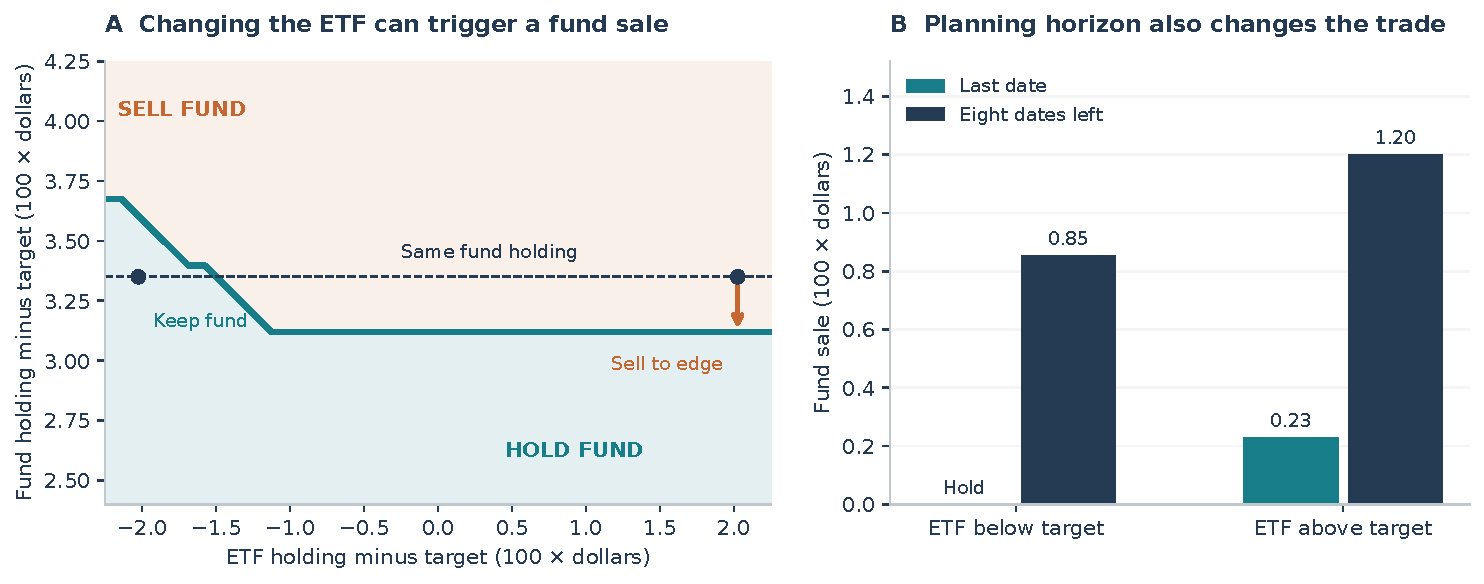
\includegraphics[width=\linewidth]{figures/fig1_bands.pdf}
\par\smallskip
\small
\phantomsection\label{fig:1}
\emph{Figure \hyperref[fig:1]{1}.} The ETF position changes the fund decision even when beliefs, costs and the fund holding are unchanged. Panel A shows the upper edge of the last-date fund hold band; the lower purchase edge is outside the displayed range. At a fund deviation of 0.0335 above target, the fund is retained with the ETF about 0.02 below its target, but sold toward the band with the ETF about 0.02 above target. Panel B applies the clipping rule to those incumbents with one or eight dates remaining. ETF deviations use the nearest available grid points. Sales and deviations are in fixed dollar units multiplied by 100, not wealth percentages. Fund rates are 10 bp each way, ETF rates 2 bp, and return-risk correlation 0.5; funding is slack. This illustrative eight-review calculation uses the moving-target specification in Appendix \hyperref[sec:C.3]{C.3}.
\end{figure}

Panel A shows why a fund cannot be assigned a trading band independently of the ETF sleeve. Panel B also shows that a longer horizon need not enlarge the region of inaction: at these inputs it leads to a larger sale. Paying a trading cost today can be worthwhile when a better allocation earns benefits over several quarters. This is an interpretation of this example, not a general theorem about how the band changes with horizon.

Free ETFs give a useful limiting reduction. If their hedge stays within their boxes for \emph{every} feasible fund holding at \emph{every} state and review, the fund problem reduces to a one-instrument dynamic band with residual-risk curvature. Feasibility only at the eventual optimizer is insufficient for this reduction. With costly ETFs, their current holdings and prospective future trades remain relevant.

\subsection{Future funding changes today's marginal values}\label{sec:4.3}

We now restore the budget and return marking. There are two reviews, one fund, one ETF and cash. Tomorrow's public state \(z\) has probability \(q(z)>0\), and each instrument has positive gross return \(g_i(z)\) between reviews. Scores use the specified state-dependent moments. Initial cash is positive, incumbents are within finite caps and sale rates are below one. These conditions define a finite concave allocation problem with nonanticipative decisions.

Let \(\eta_0\) and \(\eta_1(z)\) be cash multipliers at the two reviews, and \(t_{0,i}\), \(t_{1,i}(z)\) the trade slopes defined before Equation \hyperref[eq:12]{(12)}. Write \(g_{t,i}\) for a smooth score marginal; the two-index notation distinguishes it from the gross return \(g_i(z)\).

\phantomsection\label{res:Corollary-7}
\textbf{Corollary 7 (The value of cash and positions carried forward).} A feasible two-review policy is optimal if and only if it admits multipliers and cost slopes satisfying tomorrow's one-review conditions, cash complementary slackness at both reviews, and today's conditions

\begin{equation*}
g_{0,i}(x_0)+S_i-\hat\eta_0-(1+\hat\eta_0)t_{0,i}
\begin{cases}
=0,&0<x_{0,i}<\bar x_i,\\
\leq0,&x_{0,i}=0,\\
\geq0,&x_{0,i}=\bar x_i,
\end{cases}
\tag{23}\label{eq:23}
\end{equation*}

where

\begin{equation*}
\begin{aligned}
\hat\eta_0&=\eta_0+\beta\sum_z q(z)\eta_1(z),\\
s_i(z)&=\eta_1(z)+(1+\eta_1(z))t_{1,i}(z),\\
S_i&=\beta\sum_z q(z)g_i(z)s_i(z).
\end{aligned}
\tag{24}\label{eq:24}
\end{equation*}

The same statewise slopes and multipliers must satisfy both today's and tomorrow's conditions. If instrument \(i\) is interior tomorrow, \(s_i(z)\) equals its smooth marginal there. If it is bought, its slope is \(\kappa_i^+\); if sold, its slope is \(-\kappa_i^-\), including purchases to a cap and sales to zero.

The effective cash price \(\hat\eta_0\) includes tomorrow's expected marginal value of available cash. The incumbent value \(S_i\) credits the marked position delivered to tomorrow's problem. Both are endogenous to the same policy. Buying a position can consume flexibility through its cash requirement, while supplying flexibility through future avoided purchases or sale proceeds.

Holding the incumbent-value terms fixed, tomorrow's cash price raises today's purchase threshold by \(\beta\mathbb E[\eta_1](1+\kappa_i^+)\) and its sale threshold by \(\beta\mathbb E[\eta_1](1-\kappa_i^-)\). It also changes the incumbent values. Therefore these threshold shifts alone do not establish how the joint optimum moves. The apparent incentive to reduce one position can be offset by a larger reduction in the other.

Some useful bounds do not require the full dynamic solution. If tomorrow's off-diagonal covariance is nonnegative, each tomorrow problem admits a cash multiplier no larger than

\begin{equation*}
\bar\eta_1(z)=\max_i\frac{(\mu_{1,i}(z)-\kappa_i^+)^+}{1+\kappa_i^+}.
\tag{25}\label{eq:25}
\end{equation*}

For any admissible multiplier family, the incumbent values satisfy

\begin{equation*}
-\beta\mathbb E[g_i]\kappa_i^-
\leq S_i\leq
\beta\mathbb E[g_i\{\eta_1+(1+\eta_1)\kappa_i^+\}].
\tag{26}\label{eq:26}
\end{equation*}

These bounds are machine checked. Their quantifiers are important: a convenient multiplier selected separately in each state need not jointly support today's optimality conditions. Equation \hyperref[eq:25]{(25)} bounds some admissible multiplier in each state, not every multiplier. A binding cash constraint can have a zero multiplier, and multipliers can be nonunique. Appendix \hyperref[sec:B]{B} states a sufficient cash-coverage condition and the corresponding qualification.

For an instrument costless in both directions, Equation \hyperref[eq:24]{(24)} simplifies to \(S_i=\beta\mathbb E[g_i\eta_1]\). Its interior condition today is

\begin{equation*}
g_{0,i}=\eta_0+\beta\mathbb E[\eta_1]-\beta\mathbb E[g_i\eta_1].
\tag{27}\label{eq:27}
\end{equation*}

This is a machine-checked specialization. Even a free ETF can have a forward-looking allocation when future funding is scarce. A gross return delivered in a state with a high cash price has a different financing value from the same return delivered where cash is slack. If tomorrow's cash price vanishes in every state, this particular anticipation term disappears.

The characterization is computationally concrete: tomorrow's problems are funded one-review optimizations, and their multipliers enter today's conditions. It is not a closed-form answer based solely on today's mean and covariance. A dynamic decision needs an observation and return-transition law, not just a current estimate and error bar.

\subsection{When is repeated one-review optimization exact?}\label{sec:4.4}

Define the \emph{myopic policy}, also called repeated one-review optimization, to optimize Equation \hyperref[eq:6]{(6)} net of current costs at each date, updating beliefs and using its own carried holdings and cash. It learns at every review; what it omits is the continuation term when choosing today's action.

\phantomsection\label{res:Corollary-8}
\textbf{Corollary 8 (Testing the simpler policy).} In Corollary \hyperref[res:Corollary-7]{7}'s setting, the repeated one-review policy is dynamically optimal exactly when its initial-date allocation satisfies Equations \hyperref[eq:23]{(23)}--\hyperref[eq:24]{(24)} for some admissible multipliers and slopes of its own tomorrow problems and some admissible initial-date cash multiplier. This equivalence is machine checked, conditional on the same polyhedral optimality theorem.

For a purchase strictly inside an instrument's box, when cash is left today, a necessary initial-date consistency equation is

\begin{equation*}
S_i=\beta\mathbb E[\eta_1](1+\kappa_i^+).
\tag{28}\label{eq:28}
\end{equation*}

For an interior sale, replace \(1+\kappa_i^+\) by \(1-\kappa_i^-\). Held positions and positions at bounds instead satisfy inequalities. The equation is a necessary consistency test for this interior trade; the whole portfolio must satisfy Corollary \hyperref[res:Corollary-8]{8}.

When today's budget binds, let \(\eta_0^{\rm my}\) be a supporting cash multiplier for the one-review policy. The corresponding interior-purchase equation becomes

\begin{equation*}
S_i=(\eta_0-\eta_0^{\rm my}+\beta\mathbb E[\eta_1])(1+\kappa_i^+).
\tag{29}\label{eq:29}
\end{equation*}

An admissible nonnegative \(\eta_0\) must satisfy this equation \emph{and the other instrument's condition}. Solving for it gives a necessary inequality for this instrument, not a standalone sufficient condition for the whole portfolio. A binding budget can permit both policies to choose the same allocation on a range of inputs. It does not inevitably make one-review optimization worse.

These tests concern exactness. The economic loss from a small deviation is a separate question, addressed by common-objective policy comparisons in Section \hyperref[sec:6]{6}.

\section{Turning revised beliefs into a trading decision}\label{sec:5}

The analysis starts with the portfolio actually held and the information available at the review. An updated mean and its uncertainty enter Equation \hyperref[eq:2]{(2)} separately. A higher alpha estimate need not mean greater confidence in that estimate. A premium revision can alter the preferred use of a fund without changing the manager's alpha at all. The forecast of the next revision is another input: the same current estimate can be expected to persist, reverse or move further.

First solve the funded ETF-only problem with fund dollar positions fixed. This gives the best feasible adjustment available without changing managers. It respects the ETFs actually owned, their zero bounds, costs and the cash budget. The test in Corollary \hyperref[res:Corollary-2]{2} determines whether that ETF adjustment also solves the full one-review problem. If it fails, jointly optimize funds and ETFs. One should not infer failure or success from the ETF span alone.

Then assess continuation under the same information and mandate. Repeated one-review optimization revises beliefs and optimizes again next quarter; it is not a policy of ignoring future information. The funded two-review comparison asks whether anticipating that later optimization changes today's trade. Corollaries \hyperref[res:Corollary-7]{7}--\hyperref[res:Corollary-8]{8} identify the continuation quantities in the one-fund model. The many-instrument examples solve the full finite scenario program directly, without treating the two-instrument formulas as a general closed-form algorithm.

Three outputs should be kept separate: the current benefit from permitting a fund trade, the change in today's holdings when continuation is included, and the resulting common-horizon objective difference. A small value difference can accompany a visible portfolio change. An increased ETF balance can represent a desired factor exposure, avoided fund costs or future financing capacity; its sign alone does not identify which mechanism operates. In particular, planning can buy some funds and sell others with almost no net change in the ETF sleeve.

For an illustration intended to isolate the response to forecasts, the starting allocation must also be controlled. Section \hyperref[sec:6]{6} fixes a portfolio selected under the old beliefs and introduces news afterward. The unchanged-beliefs case measures any adjustment already warranted without that news. This is a conditional decision comparison, not a claim that every real portfolio sits exactly at a frictionless target or that historical holdings need no return marking. An illustrative funding example, in which ETF sale proceeds pay for a later fund purchase, appears in Appendix \hyperref[sec:E.1]{E.1}; it illustrates financing without claiming a planning advantage.

\section{Illustrative forecast revisions}\label{sec:6}

\subsection{Assumptions, starting portfolio and evaluation}\label{sec:6.1}

The purpose of these examples is to show which trades implement a revised forecast and why the policies differ. The inputs are hypothetical, not estimated from a fund universe. We do not interpret the resulting allocations as recommended weights or the objective differences as realized returns. Each comparison uses the same opportunity set, funding rules, information and additive quarterly objective. The relevant evidence is the response to a specified change in those inputs.

To illustrate the allocation decision, consider a manager choosing among six active funds and three ETFs supplying equity, duration and credit exposure. There are no concentration caps or prescribed sleeve weights. The sleeves have assumed quarterly excess means (1.20\%, 0.30\%, 0.60\%), return standard deviations (8\%, 3\%, 4\%), and correlations zero for equity--duration, 0.4 for equity--credit and 0.2 for duration--credit, before ETF residuals and mean uncertainty. Funds differ in their factor tilts, uncertain net alpha and residual return risk. Alpha means are (4,2,1,0.5,3,1) bp per quarter; their prior standard deviations are (20,30,10,15,15,25) bp. Appendix \hyperref[sec:C]{C} gives every loading, fee and uncertainty input. Independent fund residuals make diversification attractive; they are a modeling assumption, not an estimated cross-fund dependence structure.

The assumed ETF fees are (2,1,3) bp per quarter. At fixed factor exposure, replacing the corresponding ETF holdings with a fund saves fees: the six funds' implied fee credits are (2.10,2.15,1.10,1.15,3.10,2.85) bp per quarter. They are comparable to the assumed net alphas. Fund holdings therefore reflect alpha and avoided ETF fees, as well as residual risk, loadings and funding. A high active allocation in this example is partly built into these inputs; it is not evidence that active funds generally dominate ETFs. Alpha is already net of internal fund costs, and the fee credit is not a second estimate of manager skill.

For each old-belief configuration, select the long-only funded one-quarter optimum with investor transaction costs removed. Treat its acquisition costs as sunk and take it as the already-held portfolio. At baseline the portfolio is fully invested, with zero cash. The six fund holdings are approximately (18.6\%, 8.1\%, 12.2\%, 0\%, 30.7\%, 10.0\%) of initial wealth, and the equity ETF holds 20.5\%; the other ETFs are at zero. The risk coefficient is 2.5 with initial wealth normalized to one. It is the coefficient of this dollar-based quadratic score, not an estimated constant-relative-risk-aversion parameter. These positions are fixed before any revised forecast is supplied. No future observation is used to choose them.

Restore trading costs of 5 bp per fund purchase or redemption and 2 bp per ETF purchase or sale. Both the one-quarter optimizer and the funded two-review optimizer leave this portfolio unchanged when forecasts are unchanged, to numerical tolerance. The one-quarter control follows from construction: starting at the old costless optimum, a trade cannot improve the gross current score and adds nonnegative costs. Agreement with planning is an additional numerical finding. Together they exclude correcting an arbitrary initial allocation as the explanation for these baseline forecast responses; they do not establish that static and dynamic optima always coincide. The portfolio is not asserted to be the outcome of an optimal infinite-horizon trading history.

All policies remain unlevered and finance purchases and costs from cash or sales at every state. All observe the same public returns, use the same linear filter and can trade all instruments next quarter. The ETF-only comparison freezes funds today only. Mean persistence is 0.8, with separate state-noise variances. Persistent revisions set long-run means equal to the revised current means; reverting revisions retain the old long-run means, so 80\% of today's deviation is expected to remain at the next review. The comparisons condition on the revision and hold its current uncertainty fixed; they do not estimate a signal-generating process.

We report two distinct benefits. The \emph{current fund-trading benefit} is the joint one-review score minus the best ETF-only one-review score. The \emph{planning gain} is the funded two-review value minus the value of repeated one-review optimization, with both evaluated over the same two reviews and with optimal funded trading at the second review. Gains are expressed in bp of initial wealth: one bp is 0.0001 times starting wealth in the stipulated objective. Costs and risk charges are already deducted. Neither measure is an annualized return or a terminal-wealth certainty equivalent, and costs must not be subtracted a second time.

\subsection{Which forecast changed, and how long will it last?}\label{sec:6.2}

Consider first an equity-premium cut from 120 to 105 bp per quarter and a duration-premium increase from 30 to 35 bp, with credit unchanged. Both policies sell equity ETF and buy Duration A. The one-quarter policy moves 6.97\% of initial wealth into the fund; planning moves 8.84\%. If instead the same revision is expected to partly reverse, the one-quarter purchase is unchanged but the planning purchase is 7.86\%. Persistence affects the benefit of paying to adjust now even when the current means and their uncertainty are identical.

An alpha revision can affect whether any immediate trade occurs. Raising Equity A's quarterly alpha estimate from 4 to 9 bp leaves the one-quarter portfolio unchanged, but planning buys another 3.34\% in that fund, financed by an equity-ETF sale. Lowering alpha from 4 to -1 bp also leaves the one-quarter portfolio unchanged, while planning sells 3.79\% of the fund and buys the ETF. These are uncertain estimates, not known future returns. This comparison counts two quarters of benefits and allows a second funded decision; it ends after the second quarterly payoff, with no terminal liquidation or further continuation value.

The horizon matters to the cost-benefit comparison. Moving one dollar from an ETF into a fund costs approximately 7 bp here: a 2 bp ETF sale and a 5 bp fund purchase. That is a one-way switch; reversing it would incur another switch cost. In a simplified calculation with a fixed allocation, constant quarterly marginal benefit and a single initial cost, the undiscounted break-even benefit is that cost divided by the number of quarters. The adaptive portfolio problem also changes risk charges, holdings, future trades and funding across states. We have not established a cost-divided-by-horizon trading threshold or monotone growth of gains for that problem. The two-review examples show the shortest comparison with a subsequent decision, not the long-run value of planning. The persistence comparison has the same limitation.

An anticipated premium change with no current change produces no current trade at the baseline inputs. Proportional costs provide no mechanical cost saving from splitting a same-direction adjustment across dates, whereas quadratic costs can reward spreading trades and produce an aim ahead of the current target, as in Section \hyperref[sec:4.1]{4.1}. This helps interpret the example but is not a general no-pretrade theorem: future funding, return marking and state-dependent adjustments can make anticipation valuable even with proportional costs.

\begin{figure}[!htbp]
\centering
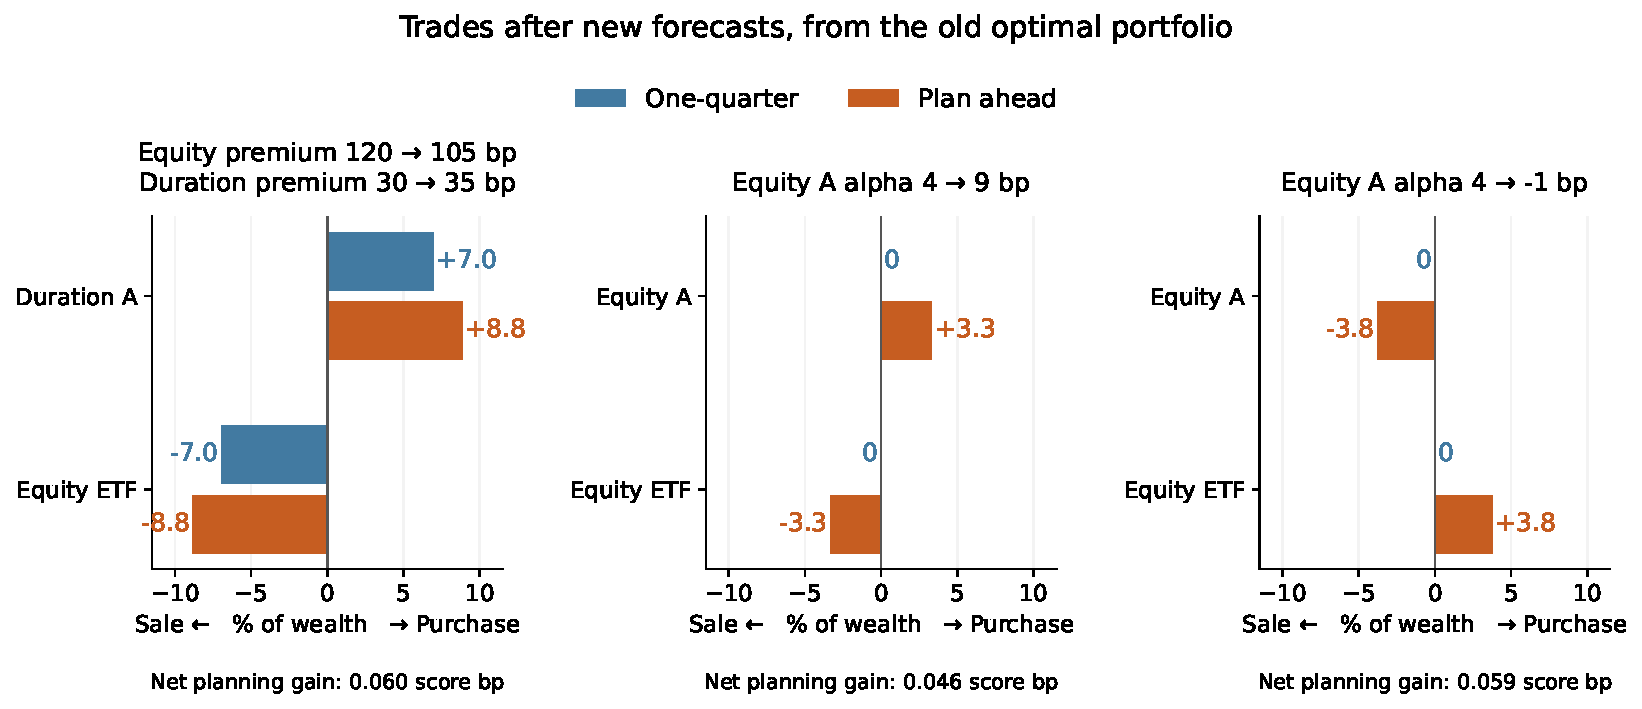
\includegraphics[width=\linewidth]{figures/fig2_forecast_revision.pdf}
\par\smallskip
\small
\phantomsection\label{fig:2}
\emph{Figure \hyperref[fig:2]{2}.} Forecast responses from the old optimal portfolio. Positive bars are purchases, negative bars sales, in percent of initial wealth. The first panel changes equity and duration premia; the other panels change only Equity A alpha. The revised means are expected to persist, with continued uncertainty and learning. Purchases and sales differ slightly because costs must be paid. All other instrument trades are numerically zero in these three cases. Under unchanged forecasts both policies make no current trade. The corresponding net two-review planning gains are only 0.060, 0.046 and 0.059 score bp of initial wealth. Thus visible trade differences coexist with small objective differences at these assumed inputs.
\end{figure}

\begin{table}[!htbp]
\centering
\parbox{\linewidth}{\phantomsection\label{tab:2}
\textbf{Table 2. Selected actions and their planning gains.} All rows start from the same old three-factor portfolio, and revised means are expected to persist. Trade amounts are percentages of initial wealth. The final column is the net two-review planning gain over repeated one-review optimization, in score bp of initial wealth. The listed actions are selected components of fully funded trades, not stand-alone purchases.}
\par\smallskip
{\footnotesize\setlength{\tabcolsep}{4pt}
\begin{tabular}{P{85pt}P{72pt}P{118pt}P{125pt}P{27pt}}
\toprule
\textbf{Revised estimate} & \textbf{ETF-only action} & \textbf{Joint one-quarter action} & \textbf{Two-review action} & \textbf{Plan gain, bp} \\
\midrule
Equity -15; duration +5 bp & Buy 6.70\% duration ETF & Buy 6.97\% Duration A & Buy 8.84\% Duration A & 0.060 \\
Equity +15; duration -5 bp & No trade & Sell 6.97\% Duration A & Sell 8.39\% Duration A & 0.036 \\
Duration +10 bp & Buy 1.24\% duration ETF & Buy 2.06\% Duration A & Buy 8.03\% Duration A & 0.262 \\
Credit +15 bp & Buy 6.12\% credit ETF & Buy 14.82\% credit ETF & Buy 9.56\% credit ETF; add credit funds & 0.307 \\
Credit -15 bp & No trade & Sell 10.03\% Credit A; 0.99\% Credit B & Sell 14.60\% Credit A; 5.80\% Credit B & 0.421 \\
Equity A alpha +5 bp & No trade & No trade & Buy 3.34\% Equity A & 0.046 \\
Credit A alpha +5 bp & No trade & No trade & Buy 1.28\% Credit A & 0.022 \\
\bottomrule
\end{tabular}}
\end{table}

The credit cases distinguish span from feasible adjustment. The menu contains a credit ETF, but the investor starts with none of it. The best ETF-only response to the credit-premium cut is no trade: it cannot sell that ETF below zero. The joint policy can instead sell credit funds, adding duration exposure and equity ETF. After the credit-premium increase, a credit-ETF purchase is feasible, and both joint policies use it. Planning also reallocates among funds. Thus a factor-premium revision can change fund holdings even though the ETF menu spans the economic factors and every alpha estimate is unchanged.

The reverse equity/duration rotation is an especially direct feasibility case. The portfolio starts with no cash, duration ETF or credit ETF. The ETF-only optimizer makes no trade: it cannot sell those absent holdings to buy more equity ETF. Joint optimization instead sells Duration A to finance the equity-ETF purchase. Other rows also involve fund sales, not simply ETF financing. After the duration-premium increase, planning finances the 8.03\% Duration A purchase by selling 5.64\% Credit A, 0.47\% Credit B and 1.93\% equity ETF. After the credit-premium increase, the one-quarter policy finances its credit-ETF purchase by selling 8.79\% Duration A and 6.03\% equity ETF. Small differences between purchases and sales pay costs. The numerical supplement provides every instrument trade for all cases.

Allocation changes and objective gains must be read together. In Figure \hyperref[fig:2]{2}'s equity/duration case, planning buys about 8.8\% of wealth in Duration A rather than 7.0\%, but improves the two-review score by only 0.060 bp. Its current transaction expenditure is 0.619 bp, versus 0.488 bp for one-review optimization. These expenditures are already included in the net comparison; the gain is not a gross benefit to be compared with an unpaid cost. The examples show that distinct allocations can have nearly equal objective values, not that these trades deliver a material performance improvement.

The budget is economically active in the three Figure \hyperref[fig:2]{2} cases. Independently solved programs have zero cash to numerical tolerance at both dates, positive root cash multipliers and positive next-review cash multipliers in every state. For the planned portfolios, the root multipliers are approximately 0.0027, 0.0028 and 0.0025, and the mean next-review multipliers are about 0.0027 in all three cases. These are marginal score values per dollar of relaxed funding, not allocation percentages or returns. They establish that future cash has marginal value at these inputs; they do not isolate how much of the planning gain is caused by funding. Appendix \hyperref[sec:C.2]{C.2} gives the normalization and verification.

These are conditional responses, not prescriptions to use active duration after every rate view or to hold less ETF when planning. Reversing the revision, changing its persistence or changing the incumbent can change the answer. The current ETF-only optimum and the fund optimality test are what determine whether an ETF adjustment suffices. The comparison distinguishes the current score gain from permitting fund trades from the additional two-review gain from planning.

The all-negative-alpha sensitivity gives a different answer. Reducing every old alpha by 5 bp leaves approximately 21.4\% in funds, primarily Credit A (14.8\%) and Equity A (5.8\%), with the remainder in ETFs. The fee credits make these slightly negative alphas compatible with a positive relative expected payoff against ETF replication; residual risk and constraints still affect the amounts. Under both directions of persistent and reverting premium rotations, neither policy trades funds: ETF trades implement the response. The alpha revisions do induce fund trades under planning. This assumed configuration illustrates when ETF adjustment suffices. It is not an estimate of the average mutual fund or of the prevalence of that outcome.

\subsection{A premium the ETFs cannot express}\label{sec:6.3}

Now add an independent, publicly observed style factor to the economic return model, while leaving the ETF menu unchanged. The factor is an attribution return, not an admissible standalone security. Its old premium is zero, return-shock standard deviation 3\% per quarter and baseline premium-estimation standard deviation 20 bp. Fund loadings are (0.5,-0.5,0,0,0.4,-0.4), in the same fund order; every ETF loading is zero. A negative style loading is a fund characteristic, not a short investor position. Alpha remains the residual expected return after all four factors, with exactly the previous alpha estimates.

Re-optimize the old portfolio with this additional factor's risk before introducing a premium revision. Its style exposure is about 0.0842 per dollar of initial wealth and its ETF allocation is 21.86\%. The factor's old zero premium does not require zero exposure, since the funds carrying it also supply alpha and other exposures. Both joint policies again leave the portfolio unchanged in the baseline no-news control.

ETF-only trades cannot change style exposure. At fixed uncertainty, revising its premium adds the same constant to the current score of every ETF-only candidate, because their fund holdings are fixed. The best ETF-only portfolio therefore remains unchanged across this revision grid. This is the zero-loading geometry of Section \hyperref[sec:3.1]{3.1}, not an inference from a small estimated correlation. By contrast, the joint optimizer can change style exposure by switching between funds with opposite loadings.

\begin{figure}[!htbp]
\centering
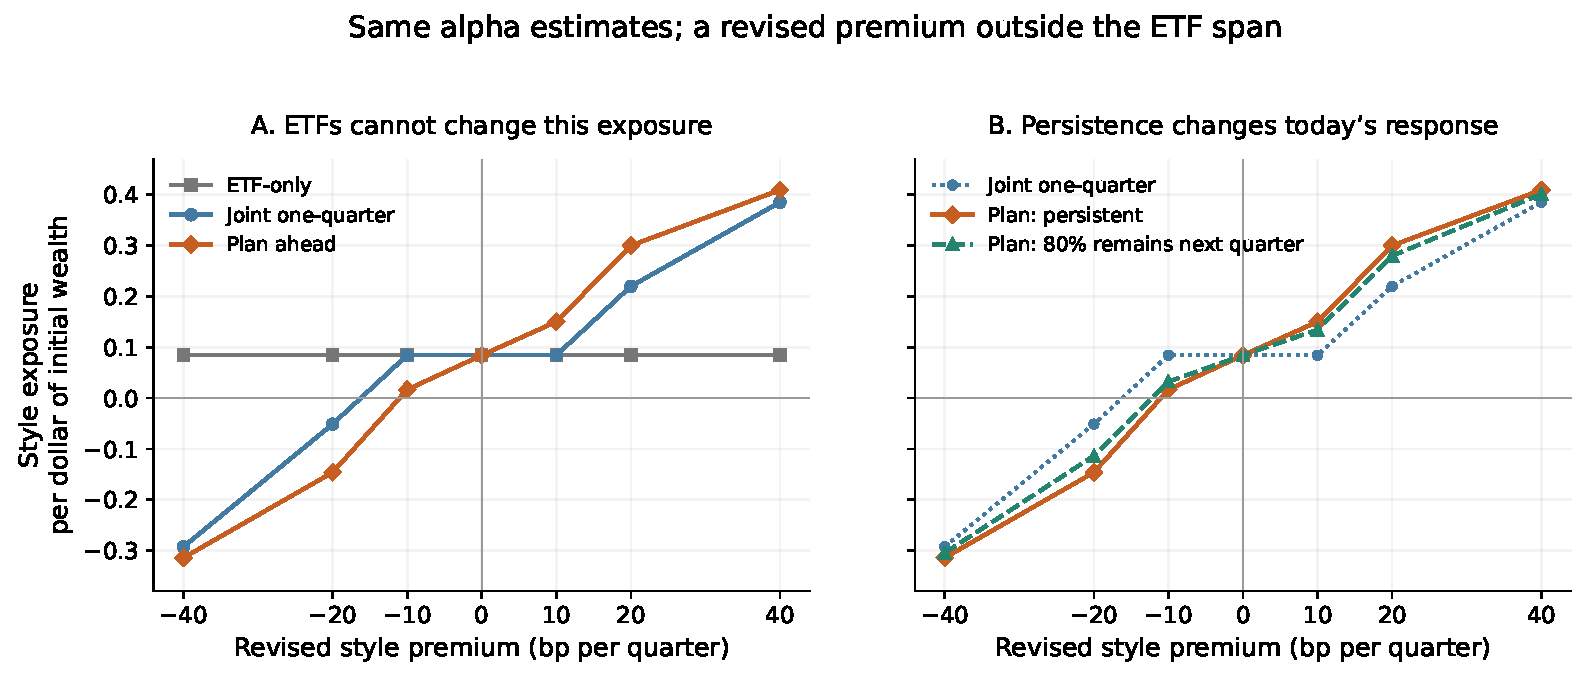
\includegraphics[width=\linewidth]{figures/fig3_unspanned_forecast.pdf}
\par\smallskip
\small
\phantomsection\label{fig:3}
\emph{Figure \hyperref[fig:3]{3}.} The missing-factor response. The horizontal axis is the revised style premium in bp per quarter, from an old estimate of zero. The vertical axis is factor exposure per dollar of initial wealth, not a capital weight. Panel A compares the ETF-only, joint one-quarter and funded planning policies for persistent revisions. Panel B holds each current revision fixed and compares planning when it persists with planning when 80\% of the revision is expected to remain next quarter. Markers are the seven solved forecasts; connecting segments guide the eye and do not estimate exact trade thresholds. All cases retain uncertain means. Neither panel represents realized performance.
\end{figure}

A revision of +10 bp leaves the one-quarter policy inside its hold region. Planning buys 2.77\% Equity A and 4.68\% Credit A, while selling 3.47\% Equity B and 3.99\% Credit B. Total ETF holdings remain essentially unchanged. With a -10 bp revision, the fund switches reverse direction. Aggregate ETF allocation would miss these responses to the factor view.

\begin{table}[!htbp]
\centering
\parbox{\linewidth}{\phantomsection\label{tab:3}
\textbf{Table 3. Unspanned-factor exposure and objective gains.} Alpha estimates are unchanged. The old exposure is 0.0842 per dollar of initial wealth; the style-premium prior SD is 20 bp, and revisions are persistent. The last two columns distinguish the current benefit of joint fund trading over ETF-only trading from the two-review benefit of planning over repeated one-review optimization. Both are score bp of initial wealth, after costs.}
\par\smallskip
{\footnotesize\setlength{\tabcolsep}{4pt}
\begin{tabular}{P{204pt}P{43pt}P{59pt}P{43pt}P{43pt}P{27pt}}
\toprule
\textbf{Premium revision} & \textbf{ETF-only exposure} & \textbf{One-quarter exposure} & \textbf{Planned exposure} & \textbf{Fund benefit, bp} & \textbf{Plan gain, bp} \\
\midrule
-20 bp & 0.0842 & -0.0514 & -0.1463 & 0.587 & 0.534 \\
-10 bp & 0.0842 & 0.0842 & 0.0165 & 0.000 & 0.284 \\
0 bp & 0.0842 & 0.0842 & 0.0842 & 0.000 & 0.000 \\
+10 bp & 0.0842 & 0.0842 & 0.1501 & 0.000 & 0.270 \\
+20 bp & 0.0842 & 0.2198 & 0.2999 & 0.587 & 0.491 \\
\bottomrule
\end{tabular}}
\end{table}

This mechanism persists as a distinction even with inexpensive ETF trading: reducing the cost of a zero-loading ETF does not give it the missing loading. But the precise trade boundary and amount depend on fund costs, alpha, other exposures and predictive risk. The additional factor's risk couples funds through their shared exposure; it must not be treated as six independent alpha changes or absorbed into estimates of manager skill. Appendix \hyperref[sec:B.2]{B.2} gives the general hedged-premium and residual-risk decomposition in its unconstrained benchmark; the portfolios here are computed with the actual funded constraints and proportional costs.

Across the 108-case forecast-revision design, the median two-review planning gain is 0.0032 bp and the maximum is 0.3917 bp. In the 49-case design covering other premia and the missing factor, the median is 0.2115 bp and the maximum is 0.5374 bp. These are summaries of deliberately selected inputs, including unchanged-beliefs controls; their medians are not estimates of a typical investor's gain. They show small incremental planning benefits in these examples despite visible allocation changes. The current benefit of trading funds is a separate quantity: it reaches 1.0935 bp in the first design and 6.3001 bp in the second. It would therefore be incorrect to describe all fund-trading benefits as fractions of a basis point. Appendix \hyperref[sec:C]{C} specifies the cases and numerical accuracy.

\section{Conclusion}\label{sec:7}

This paper studies how a manager rebalances active funds and ETFs when factor premia and fund alphas are uncertain, trading is costly and purchases must be funded. Under the stipulated quarterly mean--variance objective, the best feasible ETF adjustment provides a precise benchmark for deciding whether to change fund positions. It is jointly optimal exactly when all fund hold conditions can be satisfied with one common cash multiplier compatible with that ETF allocation.

The separation result identifies a restrictive case in which factor-premium beliefs do not enter fund selection: exact ETF spanning, no ETF fees or trading costs, slack funding and feasible interior ETF offsets, with the stated residual-risk assumptions. Outside that case, fund choice can respond to a factor-premium revision even when alpha beliefs are unchanged. The numerical illustrations distinguish a missing ETF exposure from a spanned exposure whose adjustment is blocked by a zero holding. They also show that changing factor exposure through fund substitutions need not materially change the aggregate ETF allocation.

Dynamic allocation additionally values the holdings and cash available at the next decision. The funded two-review conditions distinguish their continuation values and determine when repeated one-review optimization remains optimal. In the illustrative portfolios, anticipation can justify a current trade when one-review optimization leaves the portfolio unchanged, and forecast persistence affects the amount traded. The theory does not imply a uniform increase or decrease in ETF holdings from planning ahead.

These conclusions have explicit boundaries. The funded dynamic characterization covers two reviews with one fund and one ETF; the many-fund applications are numerical. Longer-horizon results use separate quadratic-cost or slack-funding assumptions. The analysis assumes known loadings and omits taxes, investor flows, redemption restrictions and fixed fees. Its additive quarterly objective is not a terminal-wealth criterion, and the finite-law linear filter is not generally an exact posterior. The numerical inputs are illustrative, and the two-review planning gains in the examined cases are small: visible portfolio differences do not establish a material value advantage. Alpha, ETF fees, residual dependence, forecast dynamics and the horizon all help determine those numbers. The calculations establish neither typical performance gains nor long-run allocations. The analytical tests and bounds must be evaluated using the manager's own holdings, beliefs, costs, constraints and forecast dynamics.

\clearpage
\appendix

\appsection{Proofs and scope of formal verification}\label{sec:A}

Appendix \hyperref[sec:D]{D} supplies the mathematical proofs. The finite-dimensional algebra and optimality statements have also been checked in Lean, subject to the dependencies stated below. Table \hyperref[tab:4]{4} distinguishes those results from statistical interpretations, full-policy verification arguments and numerical illustrations that are not machine checked.

Two cited mathematical inputs are carried as explicit hypotheses in the formalization: the polyhedral optimality theorem from \cite{rockafellar1970convex}, Theorems 27.4 and 28.2--28.3, and the lattice results from \cite{topkis1978minimizing}, Theorems 3.1, 3.2 and 4.3. The necessity and monotonicity conclusions identified in the table are conditional on those inputs; Lean checks their application without reconstructing the cited theorems. Gaussian and linear-filter interpretations use \cite{uhlmann2022gaussianity} and \cite{murphy2007conjugate} as cited statistical inputs. Their measure-theoretic foundations are not machine checked here.

\textbf{Availability of formal verification materials.} The accompanying formal-verification supplement (\(\texttt{formal-verification.zip}\)) contains the source snapshot, a source-to-statement guide, exact declaration excerpts and a hash manifest. The pinned toolchain is Lean 4.35.0-rc2; the Mathlib revision is \(\texttt{6ebcdee77a1b7bf10f211d4c993d85fbb19644bc}\). The guide identifies the files and declarations for each result and gives the build command. A permanent public deposit has not yet been made; an archival identifier remains required before publication.

\phantomsection\label{tab:4}
\textbf{Table 4. Proofs and verification scope.}

{\footnotesize\setlength{\tabcolsep}{4pt}
\begin{longtable}{P{84pt}lP{301pt}}
\toprule
\textbf{Statement} & \textbf{Paper proof} & \textbf{Formal scope} \\
\midrule
\endhead
\bottomrule
\endlastfoot
Proposition \hyperref[res:Proposition-1]{1} & D.1 & One-review spanning rule, caps and incumbent-sensitive trade tests \\
Corollary \hyperref[res:Corollary-2]{2} & D.2 & ETF-optimum test with one common admissible multiplier; conditional on cited polyhedral optimality \\
Proposition \hyperref[res:Proposition-3]{3} & D.3 & Scalar response and root properties in one-ETF coordinates; multiplier existence and coordinate link have paper proofs only \\
Proposition \hyperref[res:Proposition-4]{4} & D.8 & Residual loss bound and sufficient exactness; converse conditional on cited polyhedral optimality \\
Proposition \hyperref[res:Proposition-5]{5} & D.4 & Riccati and aim identities; abstract Bellman verification; Gaussian interpretation and full policy verification have paper proofs only \\
Equation \hyperref[eq:19]{(19)} & D.4 & Learning-gain bound and duration bound on the constant-state Kalman path \\
Equation \hyperref[eq:20]{(20)} & D.8 & One-step quadratic gap machine checked; expected sum has a paper proof only \\
Proposition \hyperref[res:Proposition-6]{6} & D.5 & Effective band and residual ceiling; monotonicity conditional on cited lattice results \\
Corollary \hyperref[res:Corollary-7]{7} & D.6 & Joint root and tomorrow conditions; necessity conditional on cited polyhedral optimality \\
Equations \hyperref[eq:25]{(25)}--\hyperref[eq:26]{(26)} & D.6 & Statewise multiplier bound and incumbent-value brackets with disclosed selection limits \\
Equation \hyperref[eq:27]{(27)} & D.6 & Costless-instrument specialization, including future funding \\
Corollary \hyperref[res:Corollary-8]{8} & D.7 & Multiplier-existence test, conditional on cited polyhedral optimality; interior-trade equations \\
Unspanned reduction & B.2 & Hedged-premium and residual-risk identities; unconstrained quadratic policy scope \\
Forecast-response portfolios & Section \hyperref[sec:6]{6}; C & Numerical finite programs and independent reproductions; not machine-checked policies \\
Worked funding example & E.1; C & Filter-moment identities and current moments formal; numerical policies and values computed \\
\end{longtable}}

The verification has specific limits. We do not claim that the cash-price bound can always be imposed on a joint multiplier family; that a single instrument's continuation residual determines the joint trade direction; that an interior-trade consistency equation establishes nongenericity by itself; or that the dynamic band ceiling is the actual band width. We do not transfer Gaussian posterior assertions to the finite-law filter or quadratic loss guarantees to proportional-cost funding constraints. No general closed-form many-fund, many-ETF funded dynamic policy is asserted. The finite numerical portfolio programs do not extend the scope of the stated two-instrument optimality corollaries. The additional-factor marginal in Section \hyperref[sec:3.1]{3.1} follows by differentiating Equation \hyperref[eq:2]{(2)}; it is not presented as a new theorem.

\appsection{Implementation formulas and proof structure}\label{sec:B}

\subsection{Selecting the ETF regime}\label{sec:B.1}

For Proposition \hyperref[res:Proposition-3]{3}, define the fund responses \(x_i(m,\eta)\) by Equation \hyperref[eq:14]{(14)} and let

\begin{equation*}
p(m,\eta)=\frac{\mu_E-m}{\gamma\sigma_{EE}}-\sum_i r_i x_i(m,\eta).
\tag{30}\label{eq:30}
\end{equation*}

Let \(m_0(\eta)\) solve \(p(m,\eta)=0\), and \(m_I(\eta)\) solve \(p(m,\eta)=p^-\), where \(p^-\) is the incumbent ETF holding. Set \(\theta_b=\eta+(1+\eta)\kappa_E^+\) and \(\theta_s=\eta-(1+\eta)\kappa_E^-\). For \(p^->0\):

\begin{itemize}
  \item If \(m_I>\theta_b\), the ETF is bought and \(m=\theta_b\).
  \item If \(\theta_s\leq m_I\leq\theta_b\), it is held and \(m=m_I\).
  \item If \(m_I<\theta_s\) and \(m_0>\theta_s\), it is sold to a positive holding and \(m=\theta_s\).
  \item Otherwise it is sold to zero and \(m=m_0\).
\end{itemize}

From \(p^-=0\), the ETF stays at zero when \(m_0\leq\theta_b\), and is purchased otherwise. The outer scalar search chooses the cash multiplier as in Proposition \hyperref[res:Proposition-3]{3}. The stated two-price formula requires zero ETF residual risk. With independent ETF residual variance \(v_E>0\), its marginal becomes \(m-\gamma v_Ep\), whereas the fund marginal remains \(\tilde\alpha_i+r_i m-\gamma v_i x_i^A\). Therefore the ETF purchase and sale cases solve \(m-\gamma v_Ep(m,\eta)=\theta_b\) or \(\theta_s\), rather than pinning \(m\) itself to a threshold. We retain the zero-residual-risk implementation here.

\subsection{Unspanned directions}\label{sec:B.2}

In the unconstrained quadratic benchmark, turn off ETF costs, fees and residual risk, and assume \(B^E\) has full row rank. Let \(\Pi_R\) project onto its row space and \(\Pi_U=I-\Pi_R\). With \(\tilde\Sigma=\Sigma_f+P^\lambda\), write \(\tilde\Sigma_{RR},\tilde\Sigma_{RU},\tilde\Sigma_{UR},\tilde\Sigma_{UU}\) for the projected blocks; the \(RR\) inverse acts only on the reachable subspace. Define

\begin{equation*}
\begin{aligned}
J&=\Pi_U-\Pi_R\tilde\Sigma_{RR}^{-1}\tilde\Sigma_{RU},\\
\tilde\Sigma_{U\cdot R}&=\tilde\Sigma_{UU}-\tilde\Sigma_{UR}\tilde\Sigma_{RR}^{-1}\tilde\Sigma_{RU}.
\end{aligned}
\tag{31}\label{eq:31}
\end{equation*}

The reduced fund moments are

\begin{equation*}
\alpha^{\rm red}=\hat\alpha+B^A J^\top\hat\lambda,\qquad
\Sigma^{\rm red}=\Sigma_A+P^\alpha+B^A\tilde\Sigma_{U\cdot R}B^{A\top}.
\tag{32}\label{eq:32}
\end{equation*}

These identities and the finite-dimensional policy reduction are machine checked; the Gaussian and full-policy verification steps have the same paper-level boundary as Proposition \hyperref[res:Proposition-5]{5}. If the funds' loadings lie in the reachable subspace, the premium term vanishes. We do not assert the unproved unrestricted-horizon converse about nonvanishing policy sensitivities. Equation \hyperref[eq:32]{(32)} is an unconstrained reduction, not a method of handling an ETF at zero by simply removing it once and for all.

\subsection{Computing the quadratic dynamic policy}\label{sec:B.3}

For Proposition \hyperref[res:Proposition-5]{5}, write the stacked mean as \(\mu_t=Gm_t-e\), where \(m_t\) stacks premium and alpha means, \(G\) is their loading map and \(e=(0,c^E)\). Let \(A_T=C_T=0\), \(c_T=0\), and work backward:

\begin{equation*}
\begin{aligned}
D_t&=\Lambda+\gamma\Sigma_t+\beta A_{t+1},\\
A_t&=\Lambda-\Lambda D_t^{-1}\Lambda,\\
C_t&=\Lambda D_t^{-1}(G+\beta C_{t+1}),\\
c_t&=\Lambda D_t^{-1}(\beta c_{t+1}-e).
\end{aligned}
\tag{33}\label{eq:33}
\end{equation*}

The action is

\begin{equation*}
x_t=D_t^{-1}\{\Lambda x_{t-1}+(G+\beta C_{t+1})m_t+\beta c_{t+1}-e\},
\tag{34}\label{eq:34}
\end{equation*}

and \(\Gamma_t=I-D_t^{-1}\Lambda\). This linear-quadratic recursion is machine checked. Its mean map is deterministic, its belief mean is a martingale in the baseline interpretation, and carried positions are not marked by returns. The formal setting permits positive semidefinite cost matrices, including the free-ETF separated case, while risk remains positive definite.

\subsection{Terminal fund edges beside one ETF}\label{sec:B.4}

At the last review of Proposition \hyperref[res:Proposition-6]{6}, let \((a^*,p^*)\) be the unconstrained target, \(\rho=\Sigma_{AE}/\Sigma_{EE}\), \(\rho_A=\Sigma_{AE}/\Sigma_{AA}\), and \(c^{\rm res}=\gamma(\Sigma_{AA}-\Sigma_{AE}^2/\Sigma_{EE})\). The three candidate lower edges are

\begin{equation*}
\begin{aligned}
lo_B&=a^*-(\kappa_A^+-\rho\kappa_E^+)/c^{\rm res},\\
lo_S&=a^*-(\kappa_A^++\rho\kappa_E^-)/c^{\rm res},\\
lo_I&=a^*-\rho_A(p^--p^*)-\kappa_A^+/(\gamma\Sigma_{AA}).
\end{aligned}
\tag{35}\label{eq:35}
\end{equation*}

The upper candidates replace the three final cost terms respectively by \(+(\kappa_A^-+\rho\kappa_E^+)/c^{\rm res}\), \(+(\kappa_A^--\rho\kappa_E^-)/c^{\rm res}\), and \(+\kappa_A^-/(\gamma\Sigma_{AA})\). Each actual edge is the median of its three candidates, clipped to the fund's box, provided the optimal ETF holding at that edge is strictly inside its box. These edge formulas are machine checked. An ETF bound can invalidate the median formula without invalidating the residual ceiling.

\subsection{Funding bounds and the common multiplier}\label{sec:B.5}

Under the nonnegative-covariance assumption of Equation \hyperref[eq:25]{(25)}, define tomorrow's solo purchase target and cash requirement by

\begin{equation*}
\begin{aligned}
\hat x_i(z)&=\frac{(\mu_{1,i}(z)-\kappa_i^+)^+}{\gamma\Sigma_{1,ii}(z)},\\
\mathrm{need}(z)&=\sum_i(1+\kappa_i^+)(\hat x_i(z)-g_i(z)x_{0,i})^+.
\end{aligned}
\tag{36}\label{eq:36}
\end{equation*}

If carried cash covers \(\mathrm{need}(z)\), tomorrow's problem admits a zero cash multiplier. This is a sufficient condition, not a necessary one: sales or covariance effects may reduce the actual cash requirement. If every state is covered and carried cash is strictly positive, every admissible joint family has \(\eta_1=0\). At the edge of zero carried cash and no trade, multipliers can be nonunique. Statewise choices cannot be substituted into today's conditions without checking joint compatibility. The verification includes these distinctions between multiplier selections.

The structure of Corollary \hyperref[res:Corollary-7]{7} follows by lifting purchase and sale amounts to nonnegative variables and applying the stated polyhedral optimality theorem. In the derivative with respect to today's holding, tomorrow's marked incumbent contributes \(\beta\mathbb E[g_i\{\eta_1+(1+\eta_1)t_{1,i}\}]\); today's use of future cash contributes \(-\beta\mathbb E[\eta_1](1+t_{0,i})\). Collecting these terms gives Equations \hyperref[eq:23]{(23)}--\hyperref[eq:24]{(24)}. Appendix \hyperref[sec:D.6]{D.6} gives the argument.

Similarly, Proposition \hyperref[res:Proposition-4]{4} uses the strong-supergradient bound for the optimal value at fixed exposure. Completing the square in the possible exposure change gives \(s^\top\Sigma_{EE}^{-1}s/(2\gamma)\). The residual includes the funding and zero-bound multipliers; replacing it by the ETF's unadjusted score marginal would not give the stated result.

\appsection{Illustrative analyses: assumptions and numerical methods}\label{sec:C}

All numerical inputs below are assumed. The examples illustrate the mechanisms in the theoretical results; they are neither estimates from a fund sample nor historical performance tests. Each policy comparison uses a common probability law, information set and objective. Different illustrations deliberately use different menus and trading costs, as specified below.

\subsection{Forecast revisions: portfolios and beliefs}\label{sec:C.1}

Each illustrative case begins at the old funded static optimum without investor transaction costs, independently checked with sequential quadratic programming; acquisition costs are sunk. The current review conditions on a revised estimate without historical marking of the old portfolio. Future marking is included. These are conditional comparisons, not historical backtests or simulated paths into the incumbent.

Three independent primitive factors represent correlated equity, duration and credit sleeves. ETF loading rows are (1,0,0), (0,1,0), (0.2,4/15,1); primitive means are (0.012,0.003,0.0028), shock SDs (0.08,0.03,\(\sqrt{0.00128}\)) and prior premium SDs (0.004,0.0015,0.002). ETF residual SDs are (0.001,0.0005,0.001) and quarterly fees (2,1,3) bp. Fund loading rows in ETF sleeve units are (1.05,0,0), (0.90,0.05,0.10), (0,1.10,0), (0.05,0.90,0.05), (0.05,0,1), (0,0.15,0.90). Multiplying by the ETF loading matrix gives their primitive-factor loadings. Fund residual SDs are (0.04,0.05,0.015,0.02,0.025,0.03); alpha means and prior SDs are given in Section \hyperref[sec:6.1]{6.1}. Independent fund residuals conditional on all factors are assumed.

All latent-mean persistence coefficients are 0.8. State-noise SDs are (0.001,0.0005,0.0008) for primitive premia and 0.0005 for each alpha, held fixed when initial uncertainty varies. Persistent current revisions set long-run means equal to revised means; reverting current revisions keep old long-run means. Anticipated changes keep current means unchanged and set long-run means to old means plus the desired next-review change divided by 0.2. Sleeve changes are mapped through the inverse ETF loading matrix. No future realized signal enters the current decision.

\subsection{Forecast scenarios, evaluation and numerical accuracy}\label{sec:C.2}

The first design contains 108 cases. It crosses nine forecasts with six baseline-cost configurations: \(\gamma=2.5\) and joint premium/alpha prior-SD scales 0.5,1,2; \(\gamma=2\) and \(3\) at unit scale; and \(\gamma=2.5\) at unit scale with every old alpha reduced by 5 bp. Nine forecasts comprise unchanged beliefs, both directions of persistent and reverting equity/duration rotation (an equity-premium change of -15 bp and a duration-premium change of +5 bp, or their opposites), Equity A alpha revisions of plus or minus 5 bp, and both anticipated premium rotations. The remaining 54 cases cross the same nine forecasts with six additional fund/ETF cost pairs: (0,0), (0,2), (20,2), (5,0), (5,5), (20,5) bp, at the baseline beliefs and risk coefficient. All rates are per purchase or sale. The main examples use fund/ETF costs (5,2) bp. Initial wealth is one; no caps or minimum holdings are imposed. The finite funded tree admits a redundant finite upper bound on holdings, so the numerical feasible set fits the bounded formulation without an economically binding cap.

A second design has 49 cases. Seven use the three-factor menu: unchanged beliefs, duration-premium revisions of plus or minus 10 bp, credit-premium revisions of plus or minus 15 bp and Credit A alpha revisions of plus or minus 5 bp. These revisions are persistent. The other 42 cases add the style factor specified in Section \hyperref[sec:6.3]{6.3} and cross seven current premium revisions (-40,-20,-10,0,10,20,40) bp with persistent or reverting forecasts and style-prior SDs (10,20,40) bp. Its state-noise SD is 5 bp; its return shock is independent of the original factors. All other inputs remain fixed. Duplicate zero-revision controls are retained. Old portfolios are re-optimized for each opportunity set and uncertainty specification.

Symmetric finite probability laws preserve the specified first and second moments: atoms lie on positive and negative coordinate axes at square-root-of-dimension times coordinate standard deviation, with equal probabilities on the atoms. Independent parameter and return-shock draws are then combined. The three-factor law crosses 18 parameter atoms with 24 return-shock atoms (432 states); the four-factor law crosses 20 with 26 (520 states). Gross returns are positive. Public factors and instrument returns are observed regardless of holdings. The linear filter is not the finite-law exact posterior. State noise enters the final review's predictive covariance; there is no additional observed branching date. The sums are exact for these laws, so no Monte Carlo standard error applies.

For each policy, we calculate current and future funded budgets, scores, transaction costs and expected trades. Planning gain is \(10^4(V^{\rm dyn}-V^{\rm myopic})/W_0\), a difference in the stipulated additive objective, with costs already deducted. It is not a realized return or a terminal-utility certainty equivalent. The separate current fund-trading benefit compares joint and ETF-only one-review scores. In the 108-case grid, median planning gain is 0.0032 bp and maximum 0.3917 bp; the equity/duration revision in Figure \hyperref[fig:2]{2} gives 0.0595 bp, while its two alpha revisions give 0.0461 and 0.0587 bp. These are objective gains under assumed inputs, not estimates of investment performance.

Independent numerical formulations reconstruct the state law, moments and diagonal filter and solve the portfolio programs separately. For the 108-case design, this check covers all nine baseline cases, five cost cases with solver-accuracy warnings and the maximum-gain case. Baseline gain disagreement is below 0.00000003 bp and holding disagreement below 0.00000001 of initial wealth. All 49 cases in the second design are independently reproduced: maximum holding disagreement is below 0.0000005 of initial wealth, and policy-value and gain disagreements are below 0.000003 bp. Four solver-accuracy warnings and one sequence of joint-solve retries occurred in the primary calculations for that design; the independent solves had no warnings. Budgets, transaction costs and objective values are checked from the resulting trades. These checks establish numerical agreement for the cases examined, not formal verification of the computed policies.

For the three Figure \hyperref[fig:2]{2} cases, separate vectorized quadratic programs also recover the budget multipliers. The objective is scaled by 10,000 in the solver: root duals are divided by 10,000, and next-review duals are additionally divided by their state probabilities to obtain conditional multipliers. The effective current cash price adds the expected next-review multiplier to the root multiplier, as in Equation \hyperref[eq:24]{(24)}. For the planned portfolios, next-review multiplier ranges are approximately 0.00224--0.00350, 0.00196--0.00338 and 0.00197--0.00336. The root multipliers and every next-review multiplier exceed the positivity tolerance of \(10^{-7}\); the repeated one-review policy has the same positivity classification. The largest holding disagreement with the original results is below \(10^{-8}\) of wealth and the largest objective disagreement below 0.00000008 bp. No solver warnings occurred. Multipliers can be nonunique, and these computed values do not by themselves decompose the source of a value difference. The supplement gives the selected multipliers, complete instrument trades and both objective comparisons for every case.

\subsection{Moving-target band illustration}\label{sec:C.3}

Figure \hyperref[fig:1]{1} uses an illustrative eight-review problem with one fund and one ETF, constant covariance, slack funding and no return marking of carried holdings. The risk coefficient is \(\gamma=5\) and the discount factor is \(\beta=1\). ETF return variance is \(0.0854^2\), fund return variance is \(0.0854^2+0.02^2\), and their return correlation is 0.5. Purchase and sale rates are 10 bp for the fund and 2 bp for the ETF. The target follows a symmetric finite lattice with independent positive or negative steps in its two coordinates. Each step is half the corresponding static width: for the fund the width uses its residual variance given the ETF, and for the ETF it uses its own variance. Steps are rounded to the numerical grid.

Backward dynamic programming computes the hold-band edges; the projection rule then gives the trades from the displayed incumbents. The fund deviation is 0.0335 above target, and the ETF deviations are the grid points nearest -0.02 and +0.02. The selected fund holding makes the hold/sell switch visible. Edges have finite grid resolution and are plotted without smoothing. This example prescribes target movements; it does not use the learning law of Appendix \hyperref[sec:E.1]{E.1}.

\subsection{Funding and posterior-learning illustration}\label{sec:C.4}

For the example in Appendix \hyperref[sec:E.1]{E.1} and Figure \hyperref[fig:4]{4}, independent latent means are \(\lambda\in\{0.006,0.014\}\) and \(\alpha\in\{-0.016,0.024\}\). Factor shocks are \(\{-0.084,-0.076,0.076,0.084\}\), fund-residual shocks \(\{-0.08,-0.04,0.04,0.08\}\), and ETF-residual shocks \(\{-0.005,0.005\}\). Each support is equiprobable and independent; shocks repeat independently across quarters conditional on the fixed means. The 128 hidden branches produce 72 public observations, all with positive gross returns.

The displayed ambiguous state has factor return 0.09, fund residual observation 0.064 and ETF residual shock 0.005; its probability is 0.03125. The revealing state has corresponding values 0.098, 0.104 and 0.005, with probability 0.0078125. The exact posterior is computed by grouping hidden branches with identical observations. In the posterior comparison, both policies are evaluated using prior predictive moments at review zero and true conditional posterior moments at review one. This differs from the filter manager's own score objective; the two yardsticks are not mixed in a single loss calculation.

\subsection{Comparison of allocation shortcuts}\label{sec:C.5}

The comparison in Appendix \hyperref[sec:E.2]{E.2} uses one fund and one ETF, both with factor loading one; \(\gamma=5\), \(\beta=1\), ETF fee and residual risk are zero, the fund cap is 0.25 and the ETF has no upper cap. Prior premium is 1.5\% per quarter, with standard deviation 0.5\%; factor shock standard deviation is 8\% and fund-residual shock standard deviation is 2\%. Prior alpha standard deviation is 0.35\%. Both prior standard deviations are multiplied by either one or three. The independent latent means and shocks have symmetric two-point supports, producing 16 next-review states.

The equity-style alpha mean is -0.19\%,  the ETF rate 2 bp and the baseline fund rate 50 bp. The fixed-income-style alpha mean is 0.20\%,  the ETF rate 50 bp and the baseline fund rate 20 bp. Each baseline fund rate is multiplied by 0.2, 1 or 5. Starting fund/ETF holdings are \((0,0.9)\), \((0.15,0)\), or \((0.075,0.45)\); initial cash is 0.005 or 1.0. These combinations give 72 cells, with initial wealth from 0.155 to 1.9. The cash levels deliberately contrast nearly fully invested portfolios with ample funding; their factor-of-200 difference is a design choice, not a measured liquidity distribution. Initial wealth is not held constant. The uncapped ETF can be assigned a redundant finite cap exceeding the maximum attainable wealth in this two-date tree: with \(G\) the maximum of one and all gross returns, holdings at either date are at most \(W_0G\). This gives the finite-box representation used by Corollary \hyperref[res:Corollary-7]{7} without changing a feasible trade.

When return marking takes a fund above its cap, the exposure-first first stage uses the capped fund holding and charges the mandatory sale and its cash consequences. Numerical exactness requires agreement of current and expected next-review holdings within \(10^{-5}\). Objective-loss cutoffs in Table \hyperref[tab:5]{5} are applied after normalizing by initial wealth. These policy comparisons and the multiplier-existence test are evaluated to solver tolerances; the 72 chosen cases are not a random sample of investment opportunities.

Expected transaction costs are computed from the same returns, state probabilities and instrument trades as the objective. An independent calculation reproduces every dynamic objective to numerical precision. Figure \hyperref[fig:5]{5} selects the largest loss relative to initial wealth for each shortcut across the 72 cases, so its panels illustrate failures rather than typical outcomes.

To examine whether a fixed exposure leaves room to change instruments, we intersect the fund bounds with the piecewise-linear cash inequality at each exposure-first policy state. The resulting feasible fund interval is called nearly singleton when its width is at most \(10^{-6}W_0\); thresholds of \(10^{-7}W_0\) and \(10^{-5}W_0\) give the same classification. An independent intersection of four affine cash inequalities checks all 72 initial intervals. Comparing with joint one-review optimization at the same state distinguishes a narrow feasible set from a costly restriction. Subsequent comparisons are probability weighted over near-singleton states; they do not decompose the full dynamic loss. The continuation marginal in Figure 5A and the exposure change needed to admit the joint one-review optimum in Figure 5B are calculated at the respective policy states.

\appsection{Proofs of the stated results}\label{sec:D}

These proofs use the assumptions of the corresponding statement; they do not extend a one-date, slack-funding or quadratic result to another model. Positive definiteness gives strict concavity of the smooth score. Proportional costs are convex, continuous and piecewise linear.

\subsection{Separation and the fund clipping rule}\label{sec:D.1}

Substitute the factor exposure \(y\) into the mean and covariance in Equation \hyperref[eq:2]{(2)}. With fee-free, residual-free ETFs, all factor terms depend only on \(y\); the remaining terms are the alpha mean and residual covariance of the funds. This gives Equation \hyperref[eq:9]{(9)}. At a joint optimum with slack cash and interior ETFs, arbitrary sufficiently small changes of \(y\) are feasible without changing the funds. Its first-order condition is therefore \(\hat\lambda-\gamma(\Sigma_f+P^\lambda)y=0\).

The fund block, with diagonal residual covariance, is a sum of scalar objectives

\begin{equation*}
\hat\alpha_i a-\frac{\gamma v_i}{2}a^2
-\kappa_i^+(a-a_i^-)^+-\kappa_i^-(a_i^--a)^+.
\end{equation*}

Above the incumbent its derivative vanishes at \(lo_i\); below the incumbent it vanishes at \(hi_i\). At the incumbent the two one-sided derivatives straddle zero exactly when \(lo_i\leq a_i^-\leq hi_i\). Strict concavity and the box endpoints give the two clips in Equation \hyperref[eq:10]{(10)}. The associated ETF holding follows by inversion of \(B^{E\top}\). Conversely, if this allocation is feasible, its fund and ETF conditions with zero cash multiplier establish joint optimality. This also proves the incumbent-sensitive purchase and sale tests in Proposition \hyperref[res:Proposition-1]{1}.

\subsection{The common-multiplier test}\label{sec:D.2}

For a fixed cash multiplier \(\eta\geq0\), the one-date Lagrangian is

\begin{equation*}
\mathcal L(x;\eta)=Q(x)-(1+\eta)C(x-x^-)
+\eta\{h^--\mathbf1^\top(x-x^-)\}.
\end{equation*}

Selecting \(t_i\in\partial C_i(x_i-x_i^-)\), its marginal is \(g_i-\eta-(1+\eta)t_i\). Maximizing over each box gives Equation \hyperref[eq:12]{(12)}, together with cash complementary slackness. Sufficiency follows directly: concavity bounds the objective change by this supporting linear functional; the box signs and cash feasibility make that change nonpositive.

For necessity we apply \cite{rockafellar1970convex}, Theorems 27.4 and 28.2--28.3, in the cited polyhedral form. The feasible set is an intersection of finitely many affine half-spaces: the piecewise-linear cash inequality can be written as the finite set of inequalities for its affine pieces. Equivalently, nonnegative buy and sell variables produce a linear constraint system with a differentiable concave quadratic objective. Simultaneous buying and selling is unnecessary: cancelling matched amounts preserves holdings and weakly improves both cash and the objective. Thus the cited normal-cone/multiplier result applies to a nonempty finite-dimensional convex program, without assuming a strictly positive multiplier whenever a budget binds. Strict concavity makes the risky allocation unique. The machine-checked necessity statement takes this cited polyhedral theorem as a hypothesis, as explained in Appendix \hyperref[sec:A]{A}.

At the ETF-only optimum, ETF conditions and cash complementarity already hold for an admissible set of multipliers. If one member of this set also supports every held-fund condition, it supplies the full joint KKT system, so the ETF-only portfolio is the unique joint optimum. Conversely, if the joint optimum leaves every fund unchanged, uniqueness identifies it with the ETF-only optimum; its joint multiplier supports all ETF and held-fund conditions simultaneously. This proves Corollary \hyperref[res:Corollary-2]{2}. The existential quantifier is over one common multiplier, not a separate choice for each fund.

\subsection{The two scalar prices}\label{sec:D.3}

In the coordinates of Equation \hyperref[eq:13]{(13)}, direct expansion gives

\begin{equation*}
Q(a,p)=\mu_E w-\frac\gamma2\sigma_{EE}w^2
+\sum_i\left(\tilde\alpha_i a_i-\frac\gamma2v_i a_i^2\right),
\qquad w=p+\sum_i r_i a_i.
\end{equation*}

The smooth fund marginal is \(\tilde\alpha_i+r_i m-\gamma v_i a_i\). Substitute it into Equation \hyperref[eq:12]{(12)}. The same scalar calculation as D.1 gives Equation \hyperref[eq:14]{(14)}. At a fixed cash price, the clips are continuous in \(m\), and each \(r_i a_i(m,\eta)\) is nondecreasing in \(m\), including negative \(r_i\): then both the response slope and its multiplier reverse sign. Equation \hyperref[eq:30]{(30)} is consequently continuous and strictly decreasing, with limits of opposite sign at infinity because the fund holdings are bounded. Its zero and incumbent roots are unique. Applying the ETF purchase, hold and sale conditions to these roots gives the cases in B.1.

For cash monotonicity, let \(x_j\) maximize the Lagrangian at \(\eta_j\), with \(\eta_2>\eta_1\), and write \(H(x)\) for cash after trade. Adding the two maximizing inequalities yields

\begin{equation*}
(\eta_2-\eta_1)\{H(x_2)-H(x_1)\}\geq0.
\end{equation*}

Thus cash is nondecreasing in its price. Positive initial cash makes the no-trade incumbent strictly funded; with sale rates below one, funding bounds purchases. Existence of a supporting cash multiplier follows from the cited convex optimality result. A zero-price optimum is accepted if funded; otherwise a supporting positive price has zero cash by complementarity. At either price, the scalar responses satisfy the full KKT system and hence give the unique allocation. Existence and the coordinate identification in this paragraph are paper proofs, not machine checked; the formal scalar-coordinate result takes the valid cash price as supplied.

\subsection{Quadratic dynamics and the learning bound}\label{sec:D.4}

For Proposition \hyperref[res:Proposition-5]{5}, write the value from incumbent \(z\) and belief mean \(m\) as

\begin{equation*}
V_t(z,m)=-\tfrac12 z^\top A_tz+z^\top(C_tm+c_t)+d_t(m).
\end{equation*}

The remainder \(d_t\) is independent of the incumbent. The Gaussian fixed-mean model has deterministic predictive covariance and \(\mathbb E_t m_{t+1}=m_t\); learning is independent of the action. In the Bellman maximand, collect the terms depending on the new holding \(x\):

\begin{equation*}
-\tfrac12x^\top D_tx+x^\top b_t,\qquad
b_t=\Lambda z+(G+\beta C_{t+1})m+\beta c_{t+1}-e.
\end{equation*}

The matrix \(D_t\) is positive definite because \(\gamma\Sigma_t\) is positive definite and the cost and continuation curvature are positive semidefinite. Completing the square gives the unique maximizer \(D_t^{-1}b_t\). Substitution yields Equation \hyperref[eq:33]{(33)}, starting from zero terminal coefficients. Taking \(\Gamma_t=I-D_t^{-1}\Lambda\) gives Equation \hyperref[eq:18]{(18)}. In the separated reference case the coordinate change used in D.1 makes the exposure decision costless and the fund block independent; its exposure first-order condition is the current target. Backward verification, with the Gaussian finite moments, proves optimality over measurable finite-moment policies. The matrix identities and maximization are machine checked; the conditional-expectation interpretation and measurable-policy verification are paper proofs, not machine checked.

For completeness, the scalar learning calculation can be verified directly. Write the fund's quadratic cost coefficient as \(\ell>0\), risk curvature as \(r_t=\gamma(\sigma_A^2+p_t)\), and scalar continuation curvature as \(a_t\). The recursion is

\begin{equation*}
d_t=\ell+r_t+\beta a_{t+1},\qquad
a_t=\ell-\ell^2/d_t,\qquad a_T=0.
\end{equation*}

The aim's nonnegative weights on dates \(s\geq t\) satisfy

\begin{equation*}
w_{t,t}=\frac{r_t}{r_t+\beta a_{t+1}},\qquad
w_{t,s}=\frac{\beta a_{t+1}}{r_t+\beta a_{t+1}}w_{t+1,s}\quad(s>t).
\end{equation*}

They sum to one by backward induction. Expanding the scalar affine recursion gives

\begin{equation*}
\mathrm{aim}_t=\sum_{s=t}^{T-1}w_{t,s}
\frac{\hat\alpha_t}{\gamma(\sigma_A^2+p_s)},\qquad
L_t-1=\sum_{s>t}w_{t,s}\frac{p_t-p_s}{\sigma_A^2+p_s}.
\end{equation*}

The Kalman precision identity gives \(p_s=p_t/[1+(s-t)p_t/\sigma_A^2]\), hence

\begin{equation*}
0\leq\frac{p_t-p_s}{\sigma_A^2+p_s}
\leq(s-t)\frac{p_t^2}{\sigma_A^4}
=(s-t)\left(\frac{\kappa_t}{1-\kappa_t}\right)^2.
\end{equation*}

Weighting and summing proves Equation \hyperref[eq:19]{(19)}, since \(\sum_s w_{t,s}(s-t)\leq T-1-t\). At the last date the only weight is current. As \(\ell\) tends to zero, \(0\leq a_{t+1}\leq\ell\) implies \(w_{t,t}\to1\). This proves the stated zero-cost limit. This scalar learning bound applies to the unconstrained benchmark.

\subsection{The ETF-adjusted fund band}\label{sec:D.5}

Use losses rather than rewards in this proof. Let \(V_{t+1}\) be the optimal future loss as a function of incumbent holdings and public state. It is convex in holdings by backward induction: gross marking is a positive diagonal linear map; the next-state expectation is a finite positive sum; and minimizing a jointly convex function over the fixed convex box preserves convexity. Slack funding throughout is what permits this fixed feasible box.

At a fixed current state, put

\begin{equation*}
G_t(x)=\frac\gamma2(x-x_t^*)^\top\Sigma_t(x-x_t^*)
+\beta\mathbb E_tV_{t+1}(x\mathbin{\circ}g,z'),
\qquad
U_t(a;p^-)=\min_{p\text{ in ETF box}}\{G_t(a,p)+C_E(p-p^-)\}.
\end{equation*}

Compactness and continuity give the ETF minimum. For \(d=x-x_t^*\), completing the square gives

\begin{equation*}
d^\top\Sigma_t d=
\sigma^2_{A\cdot E,t}d_A^2+
(d_E+\Sigma_{EE,t}^{-1}\Sigma_{EA,t}d_A)^\top
\Sigma_{EE,t}(d_E+\Sigma_{EE,t}^{-1}\Sigma_{EA,t}d_A).
\end{equation*}

Consequently \(U_t(a;p^-)-\gamma\sigma^2_{A\cdot E,t}(a-a_t^*)^2/2\) is convex. The remaining problem minimizes \(U_t(a;p^-)+C_A(a-a^-)\). Its one-sided derivative tests define a lower purchase edge and upper sale edge, and the unique minimizer clips the incumbent to that interval and the fund box. Across the interval, the derivative can increase by at most \(\kappa_A^++\kappa_A^-\); strong convexity requires an increase of at least \(\gamma\sigma^2_{A\cdot E,t}(hi_t-lo_t)\). This proves Equation \hyperref[eq:22]{(22)}. At a box endpoint, use the one-sided derivative pointing into the box; clipping cannot enlarge the bound.

For the monotonicity with one ETF, apply \cite{topkis1978minimizing}, Theorems 3.1, 3.2 and 4.3. Here are the hypotheses and their verification. Flip both incumbent and chosen fund coordinates to \(u=-a\), keeping the ETF coordinate \(p\). The quadratic tracking loss becomes

\begin{equation*}
-\gamma\Sigma_{AE}up+\text{terms depending on a single coordinate}.
\end{equation*}

Its cross coefficient is nonpositive when \(\Sigma_{AE}\geq0\). A convex trading cost of a difference has decreasing differences in its two arguments, including after flipping both fund arguments. Positive diagonal marking preserves the coordinate order, and expectation preserves decreasing differences. Starting from zero terminal loss, these facts make the full Bellman minimand submodular on the product of the incumbent-state and action intervals. Each interval is a chain under its usual order after the sign flip. The action box is fixed, independent of the incumbent state, so its constraint correspondence is a constant sublattice. Continuity and compactness ensure a finite attained infimum. The cited partial-minimization theorem therefore preserves submodularity backward through the horizon and when minimizing over the ETF alone.

Undoing the sign flip, \(U_t\) has increasing differences in fund holding and incumbent ETF holding. Its one-sided fund derivatives are nondecreasing in the ETF incumbent. The lower derivative-threshold crossing therefore moves left or stays fixed, as does the upper crossing. Both band edges are nonincreasing, proving the conditional monotonicity statement. This argument uses the cited lattice theorem; it does not prove that theorem anew.

At the last date the ETF optimum is its incumbent clipped between the two affine ETF thresholds. Substituting those thresholds into \(\partial G/\partial a\) gives the three increasing affine functions

\begin{equation*}
c^{\rm res}(a-a^*)-\rho\kappa_E^+,\qquad
\gamma\Sigma_{AA}(a-a^*)+\gamma\Sigma_{AE}(p^--p^*),\qquad
c^{\rm res}(a-a^*)+\rho\kappa_E^-.
\end{equation*}

The effective derivative is their median. The crossing of a fixed derivative level is the median of their crossings: at the middle crossing one function is below the level, one equal and one above. This yields B.4 when the ETF optimum is interior at each edge.

\subsection{Two-date conditions and funding bounds}\label{sec:D.6}

Write \(h_0(x_0)\) for cash after today's trade and

\begin{equation*}
h_1(z)=h_0(x_0)-\mathbf1^\top(x_1(z)-g(z)\mathbin{\circ}x_0)
-C(x_1(z)-g(z)\mathbin{\circ}x_0).
\end{equation*}

Add \(\eta_0h_0+\beta\sum_zq(z)\eta_1(z)h_1(z)\) to the two-date objective. Differentiating with respect to \(x_1(z)\), after dividing by \(\beta q(z)>0\), gives tomorrow's one-date conditions. For \(x_{0,i}\), today's terms contribute \(g_{0,i}-t_{0,i}-\eta_0(1+t_{0,i})\). Tomorrow's trade cost contributes \(\beta\mathbb E[g_i t_{1,i}]\), and tomorrow's cash constraint contributes

\begin{equation*}
\beta\mathbb E\!\left[\eta_1\{-(1+t_{0,i})+g_i(1+t_{1,i})\}\right].
\end{equation*}

Collect terms to obtain Equations \hyperref[eq:23]{(23)}--\hyperref[eq:24]{(24)}. The finite state tree has linear marking and continuous piecewise-linear costs. With the positive probabilities, positive gross returns and stated boxes, the same finite-dimensional polyhedral optimality application as D.2 supplies necessity; the Lagrangian supporting inequality supplies sufficiency. The same future slopes and multipliers occur in both derivatives, which explains the joint-selection requirement. Substitution of zero trading rates gives Equation \hyperref[eq:27]{(27)}.

For Equation \hyperref[eq:25]{(25)}, nonnegative off-diagonal covariance and nonnegative holdings imply \(g_{1,i}\leq\mu_{1,i}\). If any instrument is bought, its interior or upper-bound condition implies

\begin{equation*}
\eta_1\leq\frac{g_{1,i}-\kappa_i^+}{1+\kappa_i^+}
\leq\bar\eta_1.
\end{equation*}

If there is a sale and no purchase, cash is strictly positive and \(\eta_1=0\). If nothing trades, the admissible cash multipliers form an interval. Its lower endpoint is the maximum of zero and the purchase-threshold lower bounds for instruments below their caps, and is at most \(\bar\eta_1\). Selecting that endpoint proves existence of a bounded multiplier in each state separately. Equation \hyperref[eq:25]{(25)} is a per-state existence statement: it does not bound every multiplier or produce a family compatible with today's conditions, so the joint-compatibility caveat in Section \hyperref[sec:4.3]{4.3} applies.

For Equation \hyperref[eq:26]{(26)}, every future slope satisfies \(-\kappa_i^-\leq t_{1,i}\leq\kappa_i^+\). Therefore

\begin{equation*}
-\kappa_i^-\leq\eta_1+(1+\eta_1)t_{1,i}
\leq\eta_1+(1+\eta_1)\kappa_i^+,
\end{equation*}

where the first inequality uses \(\eta_1\geq0\) and \(\kappa_i^-<1\). Multiply by the positive weights \(\beta q(z)g_i(z)\) and sum.

Finally, in the zero-cash-price problem a bought instrument satisfies \(\gamma\Sigma_{ii}x_i\leq\mu_i-\kappa_i^+\), by the same nonnegative-covariance argument. Its purchase is bounded by the solo target in Equation \hyperref[eq:36]{(36)}. If carried cash covers the sum of those purchases including costs, the unconstrained-cash optimum is funded and hence solves the constrained problem with zero cash price. This establishes B.5's sufficient coverage condition. With strictly positive carried cash, an optimum either leaves cash or makes a purchase; in the latter case that purchase's supporting condition rules out a positive alternative multiplier at the same zero-price optimum. This gives the stated strict-cash qualification.

\subsection{Exactness of myopic optimization}\label{sec:D.7}

Tomorrow is the terminal decision, so the myopic policy already solves the relevant one-date problem from each of its own carried states. It is therefore optimal over two dates exactly when tomorrow's supporting multipliers and slopes can be selected, along with today's cash multiplier, to satisfy the remaining conditions of Corollary \hyperref[res:Corollary-7]{7}. This proves Corollary \hyperref[res:Corollary-8]{8}.

For a myopic interior purchase, \(g_{0,i}=\eta_0^{\rm my}+(1+\eta_0^{\rm my})\kappa_i^+\). Subtract this from Equation \hyperref[eq:23]{(23)} with the same purchase slope. Rearranging gives Equation \hyperref[eq:29]{(29)}. If cash is positive today, complementary slackness sets both current cash multipliers to zero, giving Equation \hyperref[eq:28]{(28)}. A sale uses slope \(-\kappa_i^-\), hence the factor \(1-\kappa_i^-\). At a held position or a bound, retain the corresponding interval or inequality. The test is simultaneous across instruments; one scalar equality is not sufficient on its own.

\subsection{Loss from fixing exposure, and the quadratic policy-loss identity}\label{sec:D.8}

For Proposition \hyperref[res:Proposition-4]{4}, let \(\mathcal V(w)\) denote the optimal one-date score at fixed exposure \(w\). In coordinates \((a,w)\), the ETF holding is \(p=w-Qa\). With residual-free spanning ETFs the smooth score splits into

\begin{equation*}
\mu_E^\top w-\frac\gamma2 w^\top\Sigma_{EE}w
+\tilde\alpha^\top a-\frac\gamma2a^\top Va.
\end{equation*}

Write \(H(a,w)\) for cash after trade and form the Lagrangian \(L(a,w)=F(a,w)+\eta H(a,w)+\zeta_E^\top(w-Qa)\), retaining the fund box as its domain. At \(x_2\), its exposure marginal is exactly \(s\) in Equation \hyperref[eq:16]{(16)}; its fund marginal is a normal to the fund box. Removing the explicit exposure quadratic leaves a function concave in the pair \((a,w)\): the fund risk term, the negative convex trading cost scaled by \(1+\eta\), and affine terms. Its concave supporting inequality at \(x_2\), together with the fund-box normal inequality, bounds the Lagrangian at any candidate allocation.

Complementarity gives \(L(x_2)=F(x_2)\). At any other feasible candidate, cash and ETF holdings are nonnegative, so \(F(a,w)\leq L(a,w)\). The multiplier terms need not vanish at that candidate; their nonnegativity is what permits this comparison. Thus, taking the optimum over feasible funds at every fundable \(w'\),

\begin{equation*}
\mathcal V(w')-\mathcal V(w_1)
\leq s^\top(w'-w_1)
-\frac\gamma2(w'-w_1)^\top\Sigma_{EE}(w'-w_1).
\end{equation*}

Take \(w'=w(x_J)\) and maximize the right side over all exposure changes. Completing the square gives Equation \hyperref[eq:17]{(17)}. If \(s=0\), the upper bound is zero and the procedure is exact. Conversely, at an exact allocation, joint KKT multipliers also support the fixed-exposure problem and make the exposure residual zero. This converse uses the cited optimality theorem. The fixed-exposure multiplier existence step is a paper proof, not machine checked. The sufficient implementation conditions in Section \hyperref[sec:3.4]{3.4} follow either from D.2's hold test or from matching ETF trade slopes and zero cash prices in the two stages.

For Equation \hyperref[eq:20]{(20)}, let \(J_t\) be the quadratic model's optimal value, evaluated at a policy's own state \(Z_t\), which includes its incumbent and beliefs. Completing the square in D.4 gives the one-step Bellman gap

\begin{equation*}
J_t(Z_t)-R_t^\pi-\beta\mathbb E_tJ_{t+1}(Z_{t+1})
=\tfrac12 e_t^\top D_t e_t,
\end{equation*}

where \(R_t^\pi\) is its current score net of cost, and \(e_t\) compares its chosen action with the Bellman optimizer at \(Z_t\). Multiply by \(\beta^t\), sum, and take expectations under that policy. The tower property cancels adjacent continuation terms, and \(J_T=0\), leaving Equation \hyperref[eq:20]{(20)}. Finite moments justify the expectations. The completed square is machine checked; this expectation-and-telescoping argument is a paper proof, not machine checked.

\appsection{Supplementary implementation diagnostics}\label{sec:E}

The following illustrative examples examine how ETF sales finance a later purchase and how specified allocation shortcuts can fail. Their initial positions and costs are deliberately illustrative. They do not isolate forecast revisions from an old optimal allocation and are not the basis of the main portfolio examples.

\subsection{ETFs as a source of future funding}\label{sec:E.1}

Consider a two-review example with a finite probability law connecting estimates, desired holdings, funding and subsequent trades. Every input is assumed. The example illustrates a decision mechanism, not a return forecast or empirical performance claim.

The fund loads 0.9 on the factor and the ETF loads 1. The ETF's quarterly fee is 5 bp. Prior mean premium is 1.0\% per quarter, with standard deviation 0.4\%; prior mean alpha is 0.4\%,  with standard deviation 2.0\%. The risk coefficient is 2.5. Observation-noise variances are 0.006416 for the factor and 0.004 for the fund residual, giving initial filter gains about 0.002488 and 1/11 respectively. Investor trading rates are 50 bp for the fund and 10 bp for the ETF, in both directions. Both dollar caps are 1. The manager initially holds 0.40 in the fund, zero ETF and 0.06 cash, in fixed dollar units. Appendix \hyperref[sec:C]{C} specifies the finite shock law.

At the first review, the frictionless target is approximately 0.406 in the fund and 0.225 in the ETF. That target is unaffordable. Both the dynamic policy and repeated one-review optimization retain the fund at 0.40 and buy 0.05994 of the ETF, spending the available cash including its purchase cost. The target, the implemented portfolio and the dynamic policy thus play distinct roles, even though the latter two coincide at the first date.

\begin{figure}[!htbp]
\centering
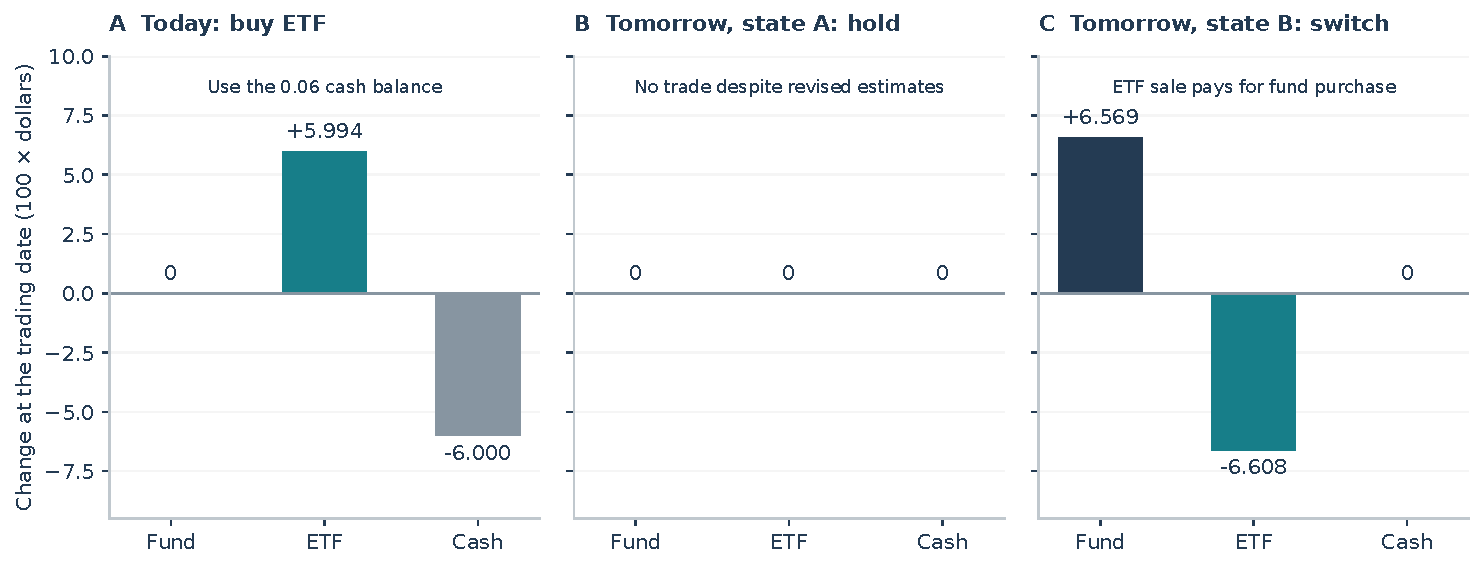
\includegraphics[width=\linewidth]{figures/fig2_worked.pdf}
\par\smallskip
\small
\phantomsection\label{fig:4}
\emph{Figure \hyperref[fig:4]{4}.} Trades, rather than total holdings. Positive bars are purchases or cash increases; negative bars are sales or cash use. All values are fixed dollars multiplied by 100. Today the fund is untouched and 0.06 cash purchases 0.05994 ETF after costs. At tomorrow's state A, no trade occurs. At state B, selling 0.0660839 ETF releases 0.0660178 after its 10 bp sale cost; this pays for 0.0656894 fund plus its 50 bp purchase cost. Before trading, the ETF is worth 0.0656044 in state A and 0.0660839 in state B because returns differ. Both dynamic and myopic optimization produce these decisions. The two tomorrow panels are alternative observations in a 72-state tree, not consecutive dates.
\end{figure}

At an ambiguous observation, the linear filter raises alpha from 0.40\% to about 0.945\%,  while the exact posterior returns to 0.40\%. Yet both managers retain the marked holdings: approximately 0.458 in the fund and 0.06560 in the ETF. The difference between those positions and yesterday's is due to returns. The uncertainty model changes the desired allocation, but the trading band and funding prevent a change in the implemented trade at this state.

At a revealing observation, the filter's alpha estimate is about 1.309\% and the exact posterior mean is 2.40\%. Both managers sell the ETF and increase the fund from its marked 0.47688 to approximately 0.54257. The fund purchase is financed by the ETF sale proceeds after transaction costs. A more optimistic estimate need not create a larger feasible purchase.

This example gives a limited but useful interpretation of ETF holdings as future adjustment capacity. The manager did not preserve cash, and the dynamic policy did not outperform the repeated one-review policy. Instead, a cheap-to-trade holding supplied both desired exposure today and sale proceeds in a state where a fund purchase was attractive tomorrow. Risky ETFs are not interchangeable with cash: their future sale proceeds depend on returns, and selling them has a cost.

The full tree also permits a separate estimation comparison. Scoring both managers with the finite law's true conditional moments, replacing the linear filter by the exact posterior improves the objective by 18.72 bp of initial wealth (0.46), entirely at the second date; actions differ in 42 of the 72 public states. The law sometimes reveals the latent mean exactly, so this is a diagnostic of posterior fidelity in this finite example. With positive prior variance and positive observation-noise variance, a single Gaussian observation leaves positive posterior variance and cannot reveal the mean exactly. The finite law is therefore an information-rich illustration; the 18.72 bp is not an upper bound or an estimate of a Gaussian-learning gain. It is also not a gain from dynamic planning. Appendix \hyperref[sec:C]{C} gives the common evaluation criterion.

\subsection{Shortcut diagnostics from arbitrary starting portfolios}\label{sec:E.2}

The policy comparison uses 72 pre-specified finite-law, two-review cases. Every policy observes the same returns, updates the same linear filter, faces the same costs and constraints, and is evaluated under the same score. The dynamic policy solves the joint two-review problem. The repeated one-review policy updates beliefs every quarter but does not anticipate future trades. The exposure-first policy applies the incumbent-aware two-stage procedure at each review. A separate frictionless first-stage procedure is evaluated only where its chosen exposure is fundable.

The cases vary initial holdings, cash, prior uncertainty, fund trading costs and two assumed regimes. The equity-style regime has negative mean net alpha and a cheap ETF; the fixed-income-style regime has positive mean net alpha and a costlier ETF. These are descriptive names for inputs, not estimates of universal asset-class differences. The design spans fund costs both above and below ETF costs. Appendix \hyperref[sec:C]{C} gives the full grid.

Define initial wealth by \(W_0=\mathbf1^\top x^-_0+h^-_0\). We report objective loss as \(10^4(V^{\rm dyn}-V^\pi)/W_0\) and trading expenditure as \(10^4\mathbb E[C(u_0)+\beta C(u_1)]/W_0\). Both are in basis points of initial wealth over the two-date problem. The former is a risk-adjusted objective difference, not a realized return or a terminal-utility certainty equivalent. Trading expenditure is already deducted in the objective; the two columns must not be added. Normalizing the reported values leaves the solved portfolios and the fixed dollar risk coefficient unchanged.

\phantomsection\label{tab:5}
\textbf{Table 5. Simpler policies evaluated on the same 72 decision problems.}

{\small
\begin{longtable}{lll}
\toprule
\textbf{Statistic} & \textbf{Myopic} & \textbf{Exposure first} \\
\midrule
\endhead
\bottomrule
\endlastfoot
Cases with loss below 0.01 bp of initial wealth & 54 of 72 & 37 of 72 \\
Numerically classified exact against dynamic policy & 24 of 72 & Not classified \\
Additional inexact cases below 0.0001 bp of initial wealth & 23 & Not classified \\
Largest objective loss, bp of initial wealth & 2.59 & 36.29 \\
Trading expenditure in that largest-loss case, bp & 21.08 & 0.06 \\
Dynamic policy's trading expenditure in the same case, bp & 24.20 & 14.71 \\
\end{longtable}}

Numerical exactness requires agreement of current and expected next-review holdings within the tolerance specified in Appendix \hyperref[sec:C.5]{C.5}. The small-loss cutoffs describe numerical magnitudes; they have no statistical significance interpretation. Initial wealth ranges from 0.155 to 1.9.

\begin{figure}[!htbp]
\centering
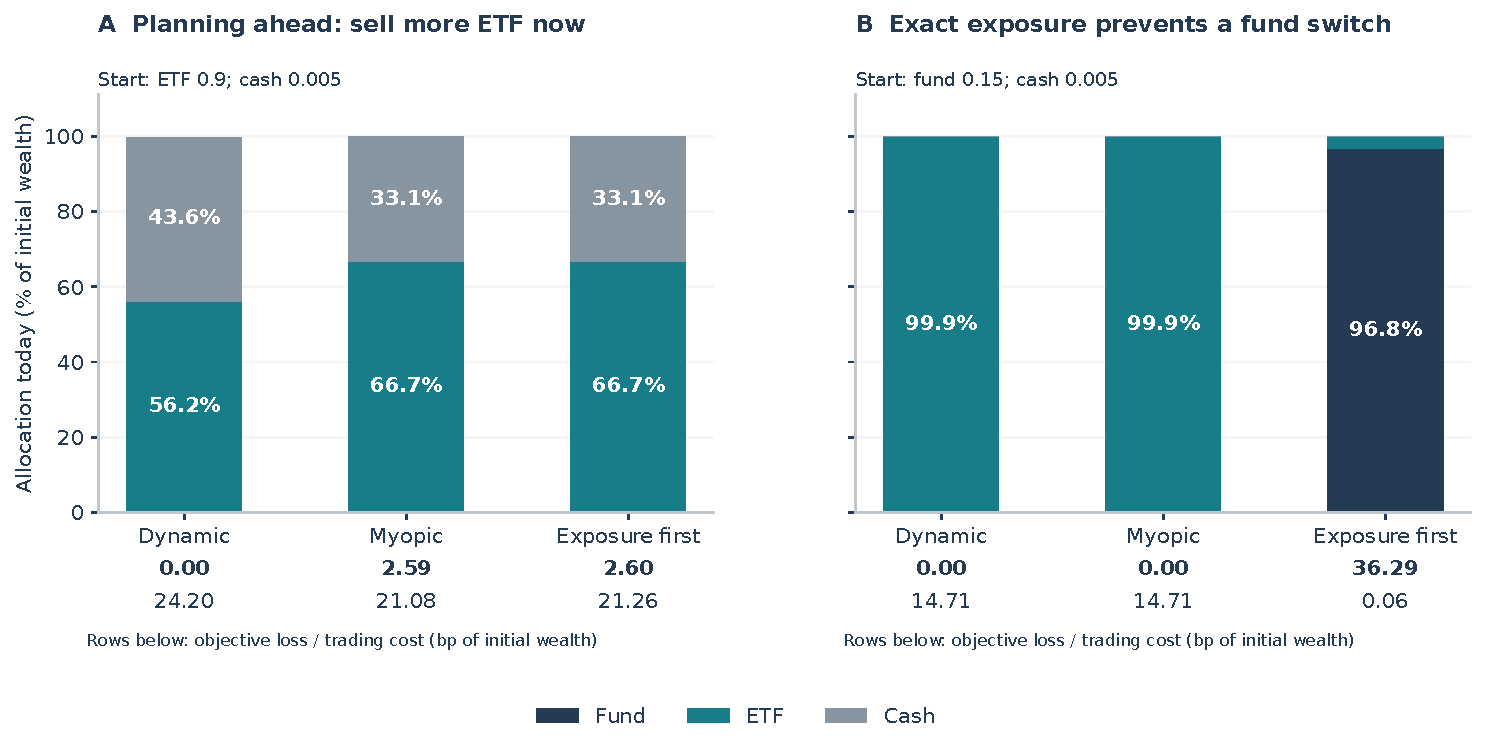
\includegraphics[width=\linewidth]{figures/fig3_policy_losses.pdf}
\par\smallskip
\small
\phantomsection\label{fig:5}
\emph{Figure \hyperref[fig:5]{5}.} The allocation behind each shortcut's largest loss relative to initial wealth. Panel A selects the largest myopic loss across all 72 cases. Panel B selects the largest loss from imposing exact first-stage exposure: spending the available cash in stage one leaves essentially a singleton feasible set in stage two. Bars show holdings and cash immediately after today's trade, divided by initial wealth; their slight shortfall from 100\% is today's trading cost. Beneath each policy are its two-date objective loss (bold) and expected two-date trading expenditure, both in bp of initial wealth. Panel A has positive mean alpha, 50 bp ETF costs and 4 bp fund costs; panel B has negative mean alpha, 2 bp ETF costs and 10 bp fund costs. Both use the higher prior-uncertainty setting. These deliberately selected failures show mechanisms, not typical outcomes; Table \hyperref[tab:5]{5} summarizes the entire grid.
\end{figure}

In panel A the dynamic policy sells the ETF down from 0.9 to 0.5083 today, whereas the myopic policy sells only to 0.6038. Tomorrow's cash multiplier is numerically zero in every state. The difference therefore concerns anticipated adjustment costs, rather than the future-funding channel in Corollary \hyperref[res:Corollary-7]{7}. After the myopic trade, tomorrow's policy sells ETF in 62.5\% of states and never buys it; favorable alpha observations also bring the fund to its cap in 25\% of states. Anticipating further ETF sales shifts today's desired ETF holding downward, so the dynamic policy brings some selling forward. At its optimum the ETF's continuation marginal is \(S_E=-0.003163\), and today's smooth marginal is \(-0.001837\): together they equal the sale slope \(-0.005\) in Equation \hyperref[eq:23]{(23)}. Anticipation need not reduce the size of the current trade.

Planning ahead spends 21.64 bp of wealth on trading today and an expected 2.56 tomorrow; myopic optimization spends 16.37 today and 4.72 tomorrow. The dynamic policy pays \emph{more} in total costs, but improves the net risk-adjusted objective by 2.59 bp. A smaller transaction bill is not the allocation objective.

In panel B joint optimization sells the entire initial fund holding of 0.15 and holds approximately 0.15482 in the ETF. The exposure-first policy freezes the fund while setting exposure and spends its initial 0.005 cash buying approximately 0.004999 ETF after costs. It then fixes that total exposure exactly. Selling any fund and buying the same dollar amount of ETF would preserve exposure but require additional transaction costs, with no cash remaining to pay them. The second-stage feasible set is essentially a singleton. The procedure retains the negative-alpha fund, and its near-zero transaction bill accompanies a 36.29 bp objective loss. Myopic joint optimization already recovers the dynamic policy here. This is a failure of the specified exact-equality procedure under an exhausted budget; it does not establish a comparable loss for procedures that allow exposure to change when selecting instruments.

Across the 72 cases, eight have a nearly singleton fixed-exposure feasible set at the initial review or a subsequent state visited by that procedure. We classify a feasible fund interval as nearly singleton when its width is at most \(10^{-6}W_0\); using \(10^{-7}W_0\) or \(10^{-5}W_0\) gives the same eight cases. Three of these cases have a one-review joint-allocation advantage exceeding 0.01 bp at the initial state or in probability-weighted subsequent near-singleton states; degeneracy alone need not cause loss. Among the other 64 cases, the largest two-date exposure-first loss is 2.60 bp. These counts describe the illustrative cases, without attributing the entire dynamic loss to a single constraint.

Relaxing the exposure equality can restore choices. In panel B, admitting today's joint one-review optimum requires an exposure tolerance of 11.61 bp of initial wealth around the first-stage exposure. This is a calculation for today's feasible set, not a demonstration that one tolerance rule reproduces the joint policy at both dates. Proposition \hyperref[res:Proposition-4]{4}'s bound does not require a non-degenerate feasible set.

The broader grid gives a mixed picture. All 15 cases with a binding budget under the dynamic policy have myopic losses below 0.001 bp of wealth; 14 are classified exact. The larger myopic losses occur in the fixed-income-style regime, whose ETF rate is always 50 bp, with tomorrow's cash prices numerically zero. From an all-ETF start, planning ahead sells more ETF today; from an all-fund start with ample cash, it buys more ETF today. Neither a binding budget nor a longer planning horizon guarantees a large policy difference. The multiplier-existence test in Corollary \hyperref[res:Corollary-8]{8} agrees with the numerical exactness classification in all 72 cases, at the stated tolerances.

\clearpage
\bibliographystyle{plainnat}
\bibliography{refs}
\end{document}
